\documentclass[10pt]{article}
\usepackage{../../_styles/preference}
\usepackage{../../_styles/math_commands}
\usepackage{cmap}

\title{Конспекты по математическому анализу}
\author{Анатолий Коченюк, Георгий Каданцев, Константин Бац}
\date{2022 год, семестр 4}

\begin{document}

\maketitle

\input{parts/lection1.tex}



\begin{theorem}
    [Фубини]

    \begin{align*}
        x = \left( x_1, \ldots, x_k \right) \\
        y = \left( y_1, \ldots, y_m \right) \\
        f(x, y) \in \mathscr L\left( E, \lambda_{k+m} \right) \\
        E\in \mathscr A_{k+m}\\
    .\end{align*}

    то:
    \begin{enumerate}
        \item Для почти всех $x\in \R^k \quad g\left( \cdot  \right)  = f\left( x, \cdot  \right) \in \mathscr L\left( E\left( x, \cdot  \right)  \right) $
        \item $I(x) = \int_{E\left( x, \cdot  \right) } f\left( x, y \right) d\lambda_m(y) \in \mathscr L\left( \R^k \right)   $\\
        \item 
            \begin{align*}
                \int_E f\left( x, y \right) d\lambda_{k+m}\left( x, y \right)  = \int_{\R^k} \left( \int_{E\left( x, \cdot  \right) } f\left( x, y \right) d\lambda_m(y) \right) d\lambda_k(x)\\
            .\end{align*}
    \end{enumerate}         
\end{theorem}

\begin{example}
    $E = A \times \{0\} \subseteq \R^{k + m} \quad_0\in \R^n$

    $A$ -- неизмеримое в  $\R^k$

    $E$ -- измеримо в  $\R^{k+m}$

    $Pr_x(E) = A$ -- неизмеримое

    Если  $Pr_x(E)$ измеримо, то вместо интеграла по $\R^k$ можно написать интеграл по проекции
\end{example}

\begin{figure}[!ht]
    \centering
    \incfig{proection}
    \caption{Переход в интегралу по проекции}
    \label{fig:proection}
\end{figure}

\begin{note}
    Если $E$ -- компактное или открытое, то  $Pr_x(E)$ измеримо.

    $Pr_x(E) = \Phi(E)$, где  $\Phi(x,y)\equiv x$ -- отображение проектирования

    Если  $E$ -- компактное, то  $\Phi(E)$ -- компактное. Если открытое, то открытое.
\end{note}

\begin{example}
    \begin{enumerate}
        \item 
            \begin{align*}
                \int_0^1dx\int_0^1 \frac{x^2-y^2}{\left( x^2+y^2 \right) ^2}dy = I_1\\
                \int_0^1dy\int_0^1 \frac{x^2-y^2}{\left( x^2+y^2 \right) ^2}dx = I_2\\
            .\end{align*}
            Если интегралы существуют, то они антиравны.

             \begin{align*}
                 I_1 = \int_0^1 \frac{y}{\left( x^2+y^2 \right) }_{y = 0}^{y = 1}dx = \int_0^1 \frac{1}{x^2+1} - 0dx = \arctg x |_0^1 = \frac{\pi}{4}
            .\end{align*}

            Вывод: функция $f(x,y) \not\in \mathscr L\left( [0,1]^2, \lambda_2 \right) $
        \item 
            \begin{align*}
                \int _{-1}^1 dx\int_{-1}^1 \frac{xy}{\left( x^2+y^2 \right) ^2}dy\\
                \int _{-1}^1 dy\int_{-1}^1 \frac{xy}{\left( x^2+y^2 \right) ^2}dx\\
            \end{align*}
            \begin{align*}
                    f\in \mathscr {L}^2\left( [-1,1]^2 \right)  \iff |f|\in \mathscr{L} \left( [-1,1]^2 \right)  \implies |f|\in \mathscr{L} \left( [-1,1]^2 \right) 
            \end{align*}
            \begin{align*}
                    \iint _{[0,1]^2} f\left( x,y \right) dy = \int _0^1 dx \int _0^1 \frac{xy}{\left( x^2+y^2 \right) ^2}dx
            \end{align*}
    \end{enumerate}
\end{example}

<.....>

\begin{statement}
    Семейство называется суммируемым, если функция суммируема 
\end{statement}

\begin{statement}
    Если семейство $\left( a_x \right)_{x\in X} $ суммируемо, то $\{x: a_x \neq 0\}$ -- не более чем счётное.
\end{statement}
\begin{proof}
    Не умаляя общности $a_x \geqslant 0$

    $+\infty  > \int_X a_xdv = \int _{X_0}a_xdv > \int a_x dv \geqslant \frac{1}{j}\nu\left( x_j \right) \implies \nu(x_j) <+\infty  $ 

    $X_0 = \bigcup\limits_{j=1}^{\infty }X_j $ -- не более, чем счётное
\end{proof}

\begin{statement}
    $\sqsupset X$ -- н.б.ч.с, $Y$ -- числовое множество,  $\left( a_x \right) _{x\in X}\subseteq Y\quad \varphi: \N  \to X$

    Тогда $\left( a_x \right) $ суммируемы $\iff \sum_{k=1}^{\infty } a_{\varphi(k)}$ сходится абсолютно.
\end{statement}

\section{Замена переменной в интеграле по мере}

\subsection{``Пересадка'' меры}

$\Phi: X \to Y$ . $\sqsupset \left( X, \mathscr A, \mu \right) $ -- пространство с мерой.

$\mathscr D = \left\{ B\subseteq Y | \Phi^{-1}(B)\in \mathscr A \right\} $

$\Phi^{-1}\left( \bigcap\limits_{k=1}^{\infty }B_k  \right) = \bigcap\limits_{k=1}^{\infty }\Phi^{-1}\left( B_k \right) \in \mathscr A $ 

$\nu\left( B \right)  = \mu\left( \Phi^{-1}\left( B \right)  \right) $ 

\begin{example}
    $X = [0,2\pi )\quad \mathscr A = \mathscr A_1 \cap [0, 2\pi )$

    $\Phi(t\in X) = \left( \cos t, \sin t \right) $
\end{example}

\begin{theorem}
    [Общая схема замены переменных]

    $\sqsupset \left( X, \mathscr A, \mu \right) \quad \left( Y, \mathscr{D}, \nu \right) $

    $\Phi: X \to Y$ -- не портит измеримость.

    $\sqsupset h\in S_+(X): \forall B\in \mathscr D$

    \[\nu(B) = \int_{\Phi^{-1}(B)}hd\mu\]

    Тогда $\forall f\in f\in S\left( Y, \nu \right)$
    \[\int_Y fd\nu = \int_X f\left( \Phi(x) \right) h(x) d\mu(x) \]
\end{theorem}
\begin{proof}
    $f\circ \Phi$ -- измерима?

    $X \left\{ f\circ \Phi < a \right\}  = \Phi^{-1}\left( Y\left\{ f<a \right\}  \right) $. $Y\left\{ f<a \right\} \in \mathscr L$, т.к. $f$ измеримо. А тогда  $\Phi^{-1}\left( \ldots \right) \in\mathscr A$ 

    Совпадение интегралов:
    \begin{enumerate}
        \item $f$ -- ступенчатая,  $f = \sum_{k=1}^{K} C_k\chi_{D_k}\quad \left\{ D_k \right\} $ -- разбиение $X$

             \begin{align*}
                 \int_Y fd\nu = \sum_{k=1}^{K} C_k \nu\left( D_k \right)  = \sum_{k=1}^{K} C_k\int_{\Phi^{-1}\left( D_k \right)} h d\mu &=  \\
                 &= \int_X \left( \sum_{k=1}^{K} C_k\chi_{\Phi^{-1}\left( D_k \right)} <?>  \right)  \\
                 &= \int_X f\circ \Phi(x)h(x)d\mu(x) \\
                 f\circ \Phi(x) = C_k\quad x\in \Phi^{-1}(D_k)\\
                 \sum_{k=1}^{K} C_k\chi_{\Phi^{-1}(D_k)}(x) = C_k
             .\end{align*}
         \item $f\in S_+(Y)\quad \exists \left\{ g_{j} \right\} $ -- ступенчатая небобратимая $g_i\uparrow f$

              \begin{align*}
                  \int_Y fd\nu = \lim_{j \to \infty} \int_Yg_jd\nu = \lim_{j \to \infty} \int_X g_j\left( \Phi(x) \right) h(x)d\mu\\
                  &= \int_X f\left( \Phi(x) \right) h(x)dmu(x).
                \end{align*}

         \item Общий случай:

             $f = f_+ + f_-$

              \begin{align*}
                  \int_Y fd\nu &= \int_Y f_+ - \int_Y f_-d\mu = \int_X f_+\left( \Phi(x) \right) h(x)d\mu(x) - \int_Y f_-\left( \Phi(x) \right) h(x)d\mu(x)\\
                  &= \int f\left( \Phi(x) \right) h(x)d\mu(x)~~~
                  \left( f\left( \Phi \right) h \right) _+ = f_+\left( \Phi \right) h
             .\end{align*}
    \end{enumerate}
\end{proof}

\begin{corollary}
    $\sqsupset \left( X, \mathscr A, \mu \right) \quad \left( Y, \mathscr D, \nu \right) $

    $h\in S_+(X);\quad \Phi:X \to Y\quad \Phi^{-1}(\mathscr D)\subseteq \mathscr A$ 

    и выполняется условие теоремы общей замены переменной. Тогда $\forall E\subseteq \mathscr D\quad f\in S\left( E, \nu \right) $:
    \[\int_E f(y)d\nu(y) = \int_{\Phi^{-1}(E) f\left( \Phi(x) \right) h(x)d\mu(x)}\]

    Рассмотрим продолжение нулём $f$ с  $E$ на  $Y$

    \[\int_E fd\nu = \int_Y (y)\chi_E(y)d\nu(y) = \int_X f\left( \Phi(x) \right) \underbrace{\chi_E\left( \Phi(x) \right)}){\chi_{\Phi^{-1}(E)}} h(x)d\mu(x) = \int_{\Phi^{-1}(E)} f\left( \Phi(x)h(x)d\mu(x) \right). \]
\end{corollary}

\begin{corollary}
    [частный случай 1]

    Если $h \equiv 1$ в условии теоремы.

    ($\forall E|in \mathscr D\quad \nu(E) = \int_{\Phi^{-1}(E)}d\mu = \mu\left( \Phi^{-1}\left( E \right)  \right) $) 

    мера $\nu$ при этом называется образом меры  $\mu$

    \[\forall  f\in S(E)\quad \int_E f d\nu  = \int_{\Phi^{-1}(E)} f\circ \Phi(x)d\mu(x)\]
\end{corollary}

\begin{corollary}
    [Частный случай 2]

    $X = Y\quad \Phi = id\quad \nu(E) = \int_E h(x)d\mu(x)$
\end{corollary}

<..>

\begin{theorem}
    $\sqsupset \left( X, \mathscr A, \mu \right) $ -- пространство с мерой, $\Phi:X \to Y\quad h\in S_+(X)$ 

    Следующие утверждения равносильны: 
    \begin{enumerate}
        \item $h$ плотность  $\nu$ относительно  $\mu$
        \item $\forall E\in \mathscr A$ \[\inf_E h \mu E \leqslant \nu(E) \leqslant  \sup_D h\mu(E)\]
    \end{enumerate}
\end{theorem}
\begin{proof}
    $I \iff \forall E\in \mathscr A\quad \nu(E) = \int_E h d\mu$

    Т.о. $I \implies II$
\end{proof}

\begin{theorem}
    [Критерий плотности]

    $\sqsupset (X, \mathscr{A})$ -- измеримое пространство, $\mu, \nu$ -- опр. (?) $\mathscr{A}$

    $h\in S_+(X)$. Тогда следующие утверждения равносильны:
    \begin{enumerate}
        \item $h$ -- плотность меры $\nu$ относительно $\mu$ ($\forall E\in \mathscr A\quad \nu(E) = \int_E hd\mu$)
        \item $\forall E \in\mathscr{A}$
        \[\inf_E h \cdot \mu(E) \leqslant d(E) \leqslant \sup_E h \cdot \mu(E) \]
    \end{enumerate}

    Если $(X, \mathscr{A}, \mu) = (\R^n, \mathcal{A}, \lambda_n)$, тогда $1 \iff 3$:
    \begin{enumerate}
        \item [3] \[\forall P\in \mathcal P_n\quad \inf_P h\cdot \mu(P) \leqslant \nu(P) \leqslant \sup_P h\cdot \mu(P)\]
    \end{enumerate}
\end{theorem}
\begin{proof}
    План: $1 \implies 2\implies 3$

    \begin{itemize}
        \item [$2\implies 1$?] $\sphericalangle E\in \mathscr{A} \quad \nu(E) \overset ? = \int_E hd\mu$

        \[E = E\left\{ h = 0 \right\} \coprod E\left\{ h = +\infty \right\} \coprod E \left\{ 0<h<+\infty  \right\} \]

        \begin{align*}
            \nu(E) &= \nu(E\left\{ h = 0 \right\}) + \nu(E\left\{ h = + \infty  \right\} ) + \nu(E\left\{ 0<h<+\infty  \right\} )\\
            \nu(E\left\{ h = 0 \right\}) &\leqslant  \sup_{E\left\{ h = 0 \right\} } = 0 = \int_{E\{h = 0\}} hd\mu\\
            \nu(E\left\{ h = + \infty  \right\} ) &\leqslant h\cdot \mu(E) + \infty \cdot \mu(E) = \int_{E\{h = +\infty \}hd\mu} 
        .\end{align*}
    \end{itemize}

    $\sphericalangle \dfrac{1}{q} \in (0, 1), ~ q >1~~~ (0, +\infty) = \bigvee\limits{k\in \Z} [q^k, q ^{k+1})$

    $E\{ h \in (0, +\infty)\} = \bigvee E \{ q^k \leqslant h < q^{k+1} \}$

    $q^k \mu(E_k) \leqslant \nu(E_k)\leqslant q^{k+1} \cdot \mu(E_k)$

    $q^k \mu(E_k) \leqslant \int h d\mu \leqslant q^{k+1} \cdot \mu(E_k)$

    $\dfrac{\nu(E_k)}{q} \leqslant q^k \cdot \mu(E_k) \leqslant \int_{E_k} h d\mu = 
    q \cdot q^{k} \mu(E_k) \leqslant q \cdot \nu(E_k)$

    Просуммируем это по всем $k$.
    
    $\dfrac{1}{q} \nu(E) = \int_E h d\mu \leqslant q \cdot \nu(E)$,~~$q \to 1 \implies$
    $\nu(E) \leqslant \int_E h d\mu \leqslant\nu(E) \implies \nu(E) = \int_E hd\mu$
    
    $\sphericalangle \tl \nu$ -- стандартное продолжение <...> (нужно дополнить)
\end{proof}

\begin{theorem}
    $\sqsupset \Phi$ -- диффеоморфизм множеств $G, O\subseteq \R^n\quad G \underset \Phi \rightarrow O$

    Тогда $\forall E\in \mathscr A_n\quad E\subseteq O$
    
    \[\lambda_n (E) = \int_{\Phi^{-1}(E)} \bigg| \det \p \Phi \bigg| d \lambda_n
    \]

    \[\lambda_n(O) = \int_G \left|\det \p \Phi  \right|d\lambda_n \]
    
    Если $O\sim \tl O\quad G\sim \tl G\quad \left( \lambda_n(O \setminus \tl O) = \O \ldots \right) $, то
    \[\lambda_n(\tl O) = \int_{\tl G} \left|\det \p \Phi  \right|d\lambda_n \]
\end{theorem}
\begin{note} % я добавлю добавил :thumbup:
    \begin{align*}
        \nu(P) \leqslant \sup_P hd\mu(P)\text{ -- от противного}\\
        \implies \exists \text{ ячейки } P_0:\quad \nu(P) > M\cdot \mu(P) = \sup_{P_0} h \cdot \mu(P)\\
        \Phi(x) = \Phi(x_0) + d_{x_0}\Phi(x - x_0) + o(x - x_0)\\
        x \approx x_0\qquad \Phi(x) \approx \Phi(x_0) + d_{x_0}\Phi(x - x_0)\\
    .\end{align*}

    Если $Q$ -- малая ячейка, то \[\lambda_n(\Phi(Q)) \approx \lambda_n d_{x_0}\Phi(Q) = \left| \det \p \Phi_{x_0} \right| \lambda_n(Q)\]
\end{note}

\begin{corollary}
    Если $\Phi: G \to O$ -- диффеоморфизм, $G, O \subseteq \R^n\quad \tl G \sim G, \tl O\sim O\quad f\in S(O)$, то 
    \[\int_{\tl O} f(x)d\lambda_n(x) = \int_{\tl G} f(\Phi(u)) \left| \det \p \Phi(u) d\lambda_n(u) \right| \]
\end{corollary}

\begin{example}
    Полярные координаты.
    
    $x = r \cos \varphi,~ y = r \sin \varphi$.
    
    $\Phi: (r, \varphi) \to (x, y)$,\\
    $([0, +\infty) \times [-\pi, \pi])) \to \R^n$,\\
    $(0, +\infty] \times (-\pi, \pi))) \to \R^n \setminus(-\infty, 0])$.

    $\det \p \Phi =r; ~~~E = \R^2: $
    \[
        \iint_E f(x, y) dx dy = \iint_{\Phi^{-1}} f(r\cos \varphi , r \sin\varphi) r dr d\varphi 
    \] 
 \end{example}

\begin{example}
    [интеграл Эйлера-Пуассона]

    \begin{align*}
        I &= \int_0^{+\infty }e^{-x^2}dx\\
        I\cdot I &= \int_0^{+\infty }e^{-x ^2}dx \cdot \int_0^{+\infty }e^{-ys} &= \iint _{\{x \geqslant 0, y\geqslant 0\}} e^{-x^2 + y^2}dxdy\\
        &= \iint_{\left\{ 0\leqslant \varphi \leqslant \frac{\pi}{2}\quad r >=0 \right\} } e^{-r^2}rdrd\varphi\\ 
        &=\int_0^{\frac{\pi}{2}}d\varphi \int_0^{+\infty }re^{-r^2}dr  \\% тут нет лишенего амперсанта? & ->  ^
        &= \frac{\pi}{2} \cdot \frac{e^{-r^2}}{-2} \mid_0^{+\infty } = \frac{\pi}{4}\\
        I = \int_0^{+\infty } r^{-x^2}dx = \frac{\sqrt \pi}{2}\\
    .\end{align*}
\end{example}

\begin{example}
    Цилиницрические координаты

    \begin{align*}
        r\cos \varphi = x\\
        r\sin \varphi = y\\
        h = z\\
    .\end{align*}

    $\Phi: (r, \varphi, h) \to (x, y, z)\quad \Phi: (0, +\infty )\times (-pi, pi)\times \R \to \R^3 \setminus \{(x, 0, z)|\mid x \leqslant 0\}\}$

    $\left| \det \p \Phi \right| = r  $

    $\iiint _E f(x, y, z)dxdydz = \iiint _{\Phi^{_1}(E)} f(r\cos\varphi, r\sin\varphi,h)\cdot rdrd\varphi dh$
\end{example}

\begin{example}
    Сферические координаты

    $r = \sqrt{x^2 + y ^2 + z^2}$
    \begin{align*}
        r\cos \varphi \cos \psi = x \\
        r\sin \varphi \cos \psi = y \\
        r\sin \psi \varphi \sin \psi = y
    \end{align*}

    $\det \p \Phi = r^2\cos\varphi$    
    
    Можно обобщить на $\R^n$

    \begin{align*}
        r = \|x\|\\
        x_1 = r\cos\varphi_{n-1}\cos\varphi_{n-2} \ldots \cos\varphi_{1}\\
        \ldots\\
        x_{n-2} = r\cos\varphi_{n-1}\cos\varphi_{n-2}\sin\varphi_{n-3}\\
        x_{n-1} = r\cos\varphi_{n-1}\sin \varphi_{n-2}\\
        x_n = r\sin\varphi_{n-1}\\
    .\end{align*}

\end{example}

\begin{example}
        \[\iiint\limits_{\substack{x^2+y^2+z^2 \leqslant \R^2\\ x^2 + y \leqslant z^2\\ z\geqslant 0}} f(x, y, z ) \,dx \,dy \,dz\]

        Преобразовать используя:
        \begin{itemize}
            \item Цилиндрические координаты

            Перепишем множество интегрирования в новых координатах:
            $\begin{cases}
                r^2+h^2 \leqslant R^2\\
                r^2\leqslant h^2 \implies r\leqslant h\\
                h\geqslant 0, r\geqslant 0
            \end{cases}$

            \begin{align*}
                I &= \iiint\limits_{\substack{r^2 + h^2 \leqslant R^2\\ r\leqslant h\\ h\geqslant 0, r\geqslant 0}} f\left( r\cos\varphi, r\sin\varphi, h \right) rdrd\varphi dh\\ 
                &= \iint\limits_{\substack{\pi \leqslant \varphi \leqslant  \pi\\ 0\leqslant r\leqslant \frac{R}{\sqrt 2}}} r \int_{r}^{\sqrt{R^2 - r^2} } f\left( r\cos\varphi, r\sin\varphi, h \right) dr \\
                &= \int_{-\pi}^{\pi}d\varphi \int_0^{\frac{R}{\sqrt 2}} rdr \int_r^{\sqrt{R^2 - r^2}} f\left( r\cos\varphi, r\sin\varphi, h \right) dh \\
            .\end{align*}

            \item Цилиндрические координаты (второй вариант)

             \begin{align*}
                 \int_0^{\frac{R}{\sqrt 2}} dh \int_{-\pi}^{\pi}d\varphi \int_0^h r fdr + \int_{\frac{R}{\sqrt 2}} dh \int_{-\pi}^{\pi}d\varphi \int_0^{\sqrt{R^2 - h^2}} rfdr\\
             .\end{align*}
            \item Сферические координаты

            $\begin{cases}
                x = r\cos\varphi\sin\psi\\
                y = r\sin\varphi\cos\psi\\
                z = r\sin\psi\\
                \tg^2 \psi \geqslant 0\\
                \sin\psi \geqslant 0\\
            \end{cases}$

            \begin{align*}
               0\leqslant r \leqslant R\\ 
                r^2\cos^2\psi \leqslant r^2\sin^2 \psi\\
                r\sin\psi \geqslant 0\\
            .\end{align*}

            \begin{align*}
                I &= \iiint_E f\left(r\cos\varphi\cos\psi, r\sin\varphi\cos\psi, r\sin\varphi  \right) r^2\cos\psi dr d\varphi d\psi \\
                &= \int_{-\pi}^{\pi}d\varphi \int_{\frac{\pi}{4}}^{\frac{\pi}{2}}d\psi \int_0^R f(\ldots)r^2\cos\psi dr \\
            .\end{align*}
        \end{itemize}
\end{example}

\begin{example}
    \[\iiiint_E z dxdydz\]

    $E:$
    \begin{align*}
       t^2(x^2 + y^2) \leqslant z^2\\
       0\leqslant z\leqslant t\leqslant 3\\ 
    .\end{align*}

    \begin{align*}
        \iiiint_E z dxdydz &= \iint_{\{0\leqslant z\leqslant t\leqslant 3\}} dzdt \iint_{\{x^2 + y^2 \leqslant \frac{4z^2}{t^2} \}} zdxdy \\
        &= \iint_{\{0\leqslant z\leqslant t\leqslant 3\}} dzdt z \pi \cdot \frac{4z^2}{z^2}\\   
        &= 4\pi \iint_{\{ 0\leqslant z \leqslant t \leqslant 3\}} \frac{z^3}{t^2}dzdt \\
        &= 4\pi \int_0^3 \frac{1}{t^2} dt \int_0^t z^3dz = \frac{4\pi}{4}\left( \int_0^3 t^2dt \right) = \pi\cdot 9  \\
    .\end{align*}


\end{example}

\section{Мера Лебега--Стилтьеса}

$\sqsupset g(x)\uparrow$ на $\R$ и непрерывна слева $\left(\lim_{x \to x_0-0} g(x) \equiv g(x_0)\right)$

\begin{problem}
    Если $h(x)$ -- произвольная возрастающая функция, то её можно превратить в непрерывную слева исправлением нбчс количества точек.

    $\exists \uparrow$ и непрерывная слева $g(x) = h(x)$ всюду кроме точек разрыва $h(x)$
    
    $g(x_0) = \lim_{x \to x_0-0}h(x) $
\end{problem}

Определим $\mu_g ([a,b]) = g(b) - g(a) \geqslant 0 $. Так же верно, что $\mu_g$ обладает счетной аддитивностью на $\mathcal P_1$ (доказывается так же, как в случае с мерой Лебега) 
$\implies \mu_g $ -- мера на $\mathcal P_1$

Стандартное продолжение $\mu_g$, которое также обозначается $\mu_g$ называется мерой Лебега-Стилтьеса, порождённой функцией $g$

\begin{align*}
    \mu_g\left( \left\{ c \right\}  \right) &= \mu_g\left( \bigcap\limits_{j=1}^{\infty }[c, c + \frac{1}{j}]  \right)  \\
    &= \lim_{j \to \infty} \mu_g\left( [c, c + \frac{1}{j}] \right)  \\
    &= \underbrace{\lim_{j \to \infty} g(c + \frac{1}{j})}_{ = g(c + 0)} - g(c) = g(c+0) - g(c)  \\
.\end{align*}

$\implies $ Если $c$ -- точка непрерывности, то $\mu_g(\{c\}) = 0$

$\mu_g ([a, b]) = \mu_g([a, b]) + \mu_g(\{b \}) = g(b) - g(a) +g(b + 0) - g(b) = \left( g(b + 0) - g(a - 0)\right)$
    
$\mu_g\left( \left( a, b \right)  \right) = \mu_g\left( [a,b)] \right)  - \mu(\{a\}) = g(b) - g(a) - (g(a + 0) - g(a)) = g(b) - g(a+0) $

$\mu_g\left( \left( a, b \right] \right) = g(b + 0 ) - g(a + 0)$

\begin{definition}
    Пусть $\mu = \sum\limits_{k=1}^\infty h_k \delta_{a_k}$,~~~
    $h_k \geqslant 0$, ~~~ $\delta_a(E) = \begin{cases}
        1,~~~ a \in E\\
        0,~~~ a \not\in E
    \end{cases}$,~~~ тогда $\mu$ --- дискретная мера.

\end{definition}

$E, E_j\in 2^{\R}\quad E = \bigvee\limits_{j=1}^{\infty }E_j \implies \delta_{a_k}(E) = \sum_{j=1}^{\infty } \delta_{a_k}(E_j)$

\begin{align*}
    \mu(E)  &= \mu(\bigvee_{j=1}^{\infty }E_j) = \sum_k\sum_j h_k\delta_{a_k}(E_j)\\
    &= \sum_j \mu(E_j)\\
.\end{align*}

Последний переход в равенстве по теореме Тонелли.

\begin{note}
    $\sqsupset \{a_k\}_{k=1}^{\infty }\subseteq \R$

    $\forall [a,b]\qquad \sum_{k: a_k\in [a,b]}h_k < + \infty $
\end{note}

\begin{example}
    Если $\{a_k\}$ -- дискретно (без точек сгущения на $\R$), то условие автоматически выполняется, т.к. перечесечения $a_k$-ых с промежутком будет конечно,
    а значит и сама сумма будет конечна

    $A = \Q\quad h_k = \dfrac{1}{2^k}$
\end{example}

\begin{definition}
    [функция Хэвисайда]
    \[\Theta(x) = \begin{cases}
        0&, x\leqslant 0\\
        1&, x>0
    \end{cases}\]

    $\sqsupset x_0\in \R\quad \forall C\in \R$

    \[g(x) = \sum_{k=1}^{\infty } h_k\cdot \left(\Theta(x - a_k) - \Theta(x_0 - a_k)\right) + C\]

    \begin{enumerate}
        \item $g(x)$ возрастает
        \item $x\in [a,b]\quad \sum_k h_k(\Theta(x - a_k) - \Theta(x_0 - a_k)) \leqslant \sum_{a_k:I_{x, x_0}} h_k$

        Разность Тет ненулевая, если $a_k$ находится между $x$ и $x_0$ -- $I_{x, x_0}$
    \end{enumerate}
\end{definition}

\begin{statement}
    $A = \{a_k\}_k$
    \begin{enumerate}
        \item $g \in C\left( \R \setminus A \right) $
        \item Непрерывность слева на $A$
    \end{enumerate}
\end{statement}
\begin{proof}
\begin{enumerate}
    \item $\sqsupset x\in \R \setminus A\quad \sqsupset (a,b)\ni x$

    $\sphericalangle \forall \varepsilon >0 \quad \sum_{k: a_k\in [a,b] } h_k < +\infty  \implies \exists K: \sum _{\substack{a_k\in [a, b]\\ k \geqslant K }} \leqslant \dfrac{\varepsilon}{2}$.
    
    $g_k (x) = h_k \left(  \Theta (x- a_k) - \Theta(x_0 - a_k)\right)$ --- локально постоянны в точке $x$ ($\exists V_{\delta}(x)~:~ g_k\mid_{V_{\delta}(x)}\equiv const$ для $k = 1, \ldots, k$)

    Не умаляя общности $[a,b] \supseteq V_{\delta}(x) $

    \begin{align*}
    g(\tl x) - g(x) &= \sum_{k=1}^{\infty } h_k\left( \Theta(x - a_k) - \Theta(x - a_k) \right) - \sum_{k=1}^{\infty }h_k \left( \Theta(\tl x - a_k) - \Theta(x_0 - a_k) \right)\\ 
    &= \sum_{k=1}^{\infty } h_k \left( \Theta(x - a_k) - \Theta(\tl x - a_k) \right)  \\
    &= \underbrace{\sum_{k=1}^{K} h_k \left( \Theta(x - a_k) - \Theta(\tl x - a_k) \right)}_{ = 0} + \underbrace{\sum_{k=K+1}^{\infty } h_k \left( \Theta(x - a_k) - \Theta(\tl x - a_k) \right)}_{ = \dfrac{\varepsilon}{2}}  \\
    .\end{align*}

    $\implies $ Непрерываность

    Если $x = a_k\quad g(x) = g_{k_0}(x) + \underbrace{\sum _{k \neq k_0}g_k}_{\text{непрерывна как в пред. случае}}$
\end{enumerate}
\end{proof}

\begin{align*}
    \mu_g\left([a,b)]  \right) &= g(b) - g(a)\\ 
    &= \sum_{k=1}^{\infty} h_k\left( \Theta(b - a_k) - \Theta(a - a_k) \right)\qquad a \leqslant  a_k \leqslant b\\
    &= \sum_{k: a\leqslant a_k < b} h_k = \mu([a,b)])\\
.\end{align*}

$\mu$ и $\mu_g$ совпадают на совокупности всевозможных промежутков.


\begin{definition}
    Пусть $f: \R \to \R$.

    Функция $f$ называется локально суммируемой  на $\R$
    $\iff \forall \, [a,b]\quad\quad f\bigg|_{[a,b]} \in \mathcal{L} (\lambda_1)$. 
\end{definition}

\begin{definition}
    $f: \R \to \R$.
    
    Функция $f$ называется абсолютно непрерывной, если существует локально суммируемая функция $h(x)$ и точка $x_0\in \R$: \[g(x) = \int_{x_0}^x h(x)d\lambda\] 
    (интеграл Лебега. Если $x < x_0$, то $\int_{x_0}^x h\, d\lambda = - \int_{[x, x_0]}h\, d\lambda$)
    
    Если $h$ непрерывна в точке $x$, то $g(x)$ дифференцируема в точке $x$ и $\p g(x) = h(x)$. Доказательство  -- смотри теорему Барроу\ldots
    
    Если $h(x) \geqslant 0$, то $g(x)\nearrow $

    Функция $g(x)$ непрерывна на $\R$. Следует из абсолютной непрерывности интеграла.

\end{definition}
\endinput

\begin{theorem}
    [воспоминание]

    \[\mu(E) = \int_{\Phi^{-1}} h d\mu \iff \forall E\in \mathscr{A} \quad \inf_E h \mu(E) \leqslant \nu(E) \leqslant \sup_E h \mu(E)\]
\end{theorem}

\begin{note}
    \[g(x) = \sum_{k=1}^{\infty } h_k \left( \Theta(x - a_k) - \Theta(x_0 - a_k) \right) \]

    Для этой меру нужно было фиксировать открытый интервал $\Delta$, что \[ \forall [a,b] \subseteq \Delta\quad \sum_{k: a_k\in [a,b]}h_k < +\infty  \]

    \begin{align*}
       g(a_k + 0) - g(a_k - 0) &= h_k\left( \Theta(a_k - a_k + 0) - \Theta(x_0 - a_k + 0) - \Theta(a_k-a_k - 0) + \Theta(x_0 -a_k - 0) \right)  \\ 
       &= h_k \\ %?
    .\end{align*}
\end{note}

\begin{statement}    
Если $\nu = \sum\limits_k h_k \delta_{a_k}$, то $\nu$ совпадает с $\mu_g$ на $\mathscr{A}_{\mu_g}$ при условии (*).
\end{statement}
\begin{proof}

    Если хочется скорее сослаться на теорему об единственности, то можно сделать так:    
    Рассмотрим $[a, b)$. $\nu([a, b)) = \sum\limits_{k \,:\, a_k \in [a, b)} h_k.$

    \[ \mu_g([a, b)) = g(b) - g(a) = \sum_{k\in\N} h_k \left(\Theta(b - a_k) - \Theta(a - a_k)\right) = \sum_{k \,:\, a_k \in [a, b)} h_k.\]

    Если $\{ a_k\}_k$ --- конечное множество, то вопросов с суммируемостью не веознкает.

    \[g(x) = \sum_k h_k \cdot \Theta(x - a_k) + C   \]
\end{proof}

\begin{note}
    Локально суммируемая функция -- это такая, что она будет на любом шаре суммируемой по Лебегу
\end{note}

\begin{theorem}
    $g(x)$ -- абслолютно непрерывная $\iff \exists h\in \mathscr L_{loc}\left( \R, \lambda \right) \exists x_0\in \R, c\in \R$ 
    \[(x) = \int_{x_0}^x h(x) d\lambda + C\]
\end{theorem}  

По теореме Барроу $g(x)$:
\begin{itemize}
    \item $g(x)\in C(\R)$,
    \item $g(x)$ дифференцируема в точках ... функции $h(x)$. 
\end{itemize}

\begin{proof}
\begin{itemize}
    \item  Если $x_1\in \R$ \[g(x) - g(x_1) = \int_{x_1}^x h(x)dx\]

$\exists \delta_0 >0, x\in V_{\delta_0}(x_1), \quad h\in \mathscr L\left( V_{\delta_0} \right) $

$\forall \varepsilon >0 \exists \delta (\leqslant \delta_0 ) >0 : \int_E h(x)d\lambda  < \varepsilon \forall E\subseteq V_{\delta_0}(x_1):\, \lambda_1(E) <\delta$

$\implies $ Если  $\left| x_1 - x \right| <\delta\quad \left| \int_{x_1}^x h(x)dx \right| \leqslant \varepsilon$

\item Пусть $x_1$ --- точка непрерывности для $h(x)$. $h(x) = h(x_1) + \underbrace{ \alpha (x - x_1)}_{o(1) \text{ при } x\to x_1 }$

\[ \dfrac{g(x) - g(x_1)}{x - x_1} = \frac{1}{x - x_1} \int_{x_1}^x h(x_1) + \alpha(x-x_1)dx = h(x_1) + \frac{1}{x - x_1} \int_{x_1}^x \alpha(x - x_1)dx \leqslant \varepsilon(x - x_1)\]

Если ``$x$ остаточно близок к $x_1$''
\end{itemize}
\end{proof}

\begin{note}
    В частности, если $h(x) \in C(\R) \implies g\in C^1(\R)$ и $\p g(x)\equiv h(x)$    
\end{note}

\begin{note}
    \[\int_E fd\nu = \sum_{k\,:\,a_k\in E} h_k f(a_k) = \sum_{k\,:\,a_k\in E} f(a_k) \cdot \text{ скачок } g(a_k)\]  
\end{note}

\begin{statement}
    $\sqsupset g(x) = \int_{x_0}^x h(x)d\lambda_1(x) +C\quad h(x) \geqslant 0\quad h\in \mathscr{L}_{loc}\left(  \R, \lambda\right) $     абсолютно непрерывная возрастающая функция.
  
    Тогда $\int_E f d \mu_g = \int_E f(x) h(x) d \lambda (x)$.

    В частности, $\forall$~возрастающей $g(x) \in C^{1} (\R)$.
    \[\int_E f d\mu_g = \int_E f \cdot \p g (x) d \lambda(x) \left( = \int_E f \cdot dg \right). \]
\end{statement}

\begin{proof}
    $\sphericalangle \nu (E) = \int_E h d \lambda_1$. 
    \[\mu_g (\langle a, b \rangle )= \mu_g ([a, b)) = g(b) - g(a) = \int_a^b h(x) d \lambda_1 = \nu([a, b)) = \nu(\langle a, b \rangle ). \]

    $\mu_g$ и $\nu$ совпадают на открытых. Если $K$ -- компакт, $K = B \setminus \left( B \setminus K  \right) $

    $\nu(K) + + \nu(B \setminus K) = \nu(B)\qquad \mu_g(K) = \nu(K) = \nu(B) - \nu(B \setminus K)$

    $\sqsupset E$ -- $\lambda_1$-мера $O$

    $ \implies \exists \delta >0 \exists $ открытое $G: E\subseteq G$ и $:\lambda_1(G) <\delta$
    
    
    $\implies \int\mid_{G_0}$ -- абсолютно непрерывное $\implies \forall \varepsilon>0 \exists \delta>0: \lambda_1(\tl E)<\delta\quad \tl E \subseteq G$
    
    $\int_{\tl E}h < \varepsilon\quad \tl E = G \implies \nu(G) <\varepsilon \implies \mu_g(G) <\varepsilon\,\varepsilon\text{ --- } \forall  \implies \nu(E) = \mu_g(E) = 0$   

    Если $E$~--- неограничено $\lambda_1$--меры 0 $\implies \exists~$ ограниченное $E_j\,:\,E=\bigcup E_j$.
    $\forall i \in \N ~ \lambda_1 (E_j) = 0 \implies \nu(E_j) =\mu_g (E_j) = 0$ $\implies \nu(E) = \mu_g (E).$

    Дальше можно применить теорему о плотности меры. Применяю общую мхему замены переменной все доказывается. 
\end{proof}
\begin{problem}
    \begin{enumerate}
        \item $g(x) = \arctg x$. Найти:
        \begin{enumerate}
            \item $\sup \Bigg\{ \mu_g(I)~:~ I = \langle a, b \rangle,~ \lambda_1 (I) \leqslant \delta \Bigg\},~ \delta > 0$.
            \item $\sup \Bigg\{ \lambda_1(I)~:~ I = \langle a, b \rangle,~ \mu_g (I) \leqslant \delta \Bigg\},~ \delta > 0$.
        \end{enumerate}
        \item $g(x) = \arctg x + \Theta(x - 1)$
        \begin{enumerate}
            \item Для $\delta = 1$
        \end{enumerate}  
    \end{enumerate}
\end{problem}
\begin{proof}
    [Решение]

    $\mu_g(I) = g(b) -g(a) = \int_I \p g(t)dt = \int_{[a,b]}\frac{dt}{1 + t^2}$

    \begin{enumerate}
        \item 
        \begin{enumerate}
            \item \begin{align*}    
                \sup \{\mu_g(I)\} &= 2 \int_0^{\frac{\pi}{2}} \frac{dt}{1 + t ^2}\\
            .\end{align*}
        \end{enumerate}
    \end{enumerate}
\end{proof}

\begin{example}
    Пример меры Лебега--Стилтьеса 
    не евклидовой, не дискретной, не абсолютно непрерывной:

    \begin{align*}
        C_0 &= \left[0,1\right]\\
        C_1 &= \left[0, \frac{1}{3}\right] \cup \left[\frac{2}{3}, 1\right] \\
        C_2 &= \left[0, \frac{1}{9}\right] \cup \left[\frac{2}{9}, \frac{1}{3}\right] \cup \left[\frac{2}{3}, \frac{7}{9}\right] \cup \left[\frac{8}{9}, 1\right]  \\
        C_{k+1} &\subseteq C_k\quad C_k \text{ -- компакт}\\
        C &= \bigcap\limits_{k=1}^{\infty}C_k \text{ -- компакт}  \\
        \lambda_1(C) &= \lambda_1([0,1]) - \frac{1}{3} - \frac{2}{9}  - \ldots - \frac{2^{k-1}}{3^k} = 0\\
    .\end{align*}  

    $\psi(x) = \frac{1}{3}x\quad \Theta(x) = 1-x$
    
    \[\Phi = \left\{ [0,1] \cap C, \psi(C), \Theta\psi(C), \psi \psi(C), \psi\Theta(C), \Theta\psi\psi(C) , \Theta\psi\Theta\psi(C), \ldots \right\} \] 
    -- полукольцо

    $\mu(C) = 1\quad \mu(P) = \frac{1}{2^k}$ -- если $P$ есть результат применения $k$ штук $\psi$ и $\Theta$

    $\sphericalangle \mu$ -- стандартное продолжение
\end{example}
\section{Г-функция Эйлера}

\begin{definition}
    $\Gamma(p) = \int_0^{+\infty }x^{p-1}e^{-x}dx$

    $p >0$
\end{definition}

\begin{property}
    \[\Gamma(p+1) = p\Gamma(p)\quad \forall p >0\] -- формула приведения

    \[\Gamma(p) = \frac{\Gamma(p+1)}{p}\] -- определение для $\Gamma$ в $\R\setminus \left( \Z_- \right) $

    \begin{align*}
    \Gamma(1) &= 1\quad \Gamma(p + 1) = p!\\
    \Gamma(\frac{1}{2}) &= \frac{e^{-x}}{\sqrt{x}}dx = 2\int_0^{+\infty }e^{-t^2}dt = 2 \cdot \frac{\sqrt{\pi}}{2} = \sqrt{\pi}\\
    \Gamma(\frac{3}{2}) &= \frac{1}{2} \Gamma(\frac{1}{2}) = \frac{\sqrt{\pi} }{2}\\
    \Gamma(\frac{5}{2}) &= \frac{3\sqrt{\pi} }{4}\\
    \Gamma(\frac{2n+1}{2}) &= \frac{(2n-1)!!}{2^n} \sqrt{\pi} \text{(по индукции)}\\
    .\end{align*}
\end{property}

\begin{note}[Дифиренцирование $\Gamma$--функции]
    \[
    \Gamma^{(k)}(p) = \int_0^{+\infty } \underbrace{x^{p-1}e^{-x} \left( \ln x \right) ^k}_{f_k(x, p)} dx
    .\] 

    $\frac{\partial f_k(x, p)}{\partial p} = f_{k+1}(x, p)$
\end{note}

\begin{note}
    Локальное условие Лебега $\forall p_0$?

    \[
    \exists V_{p_0}: \exists \Phi(x) \in \mathcal L \left( \left( 0, +\infty  \right): \left| f_k(x, p) \right| \leqslant \Phi(x)  \right) 
    .\] 

    \begin{align*}
        x^{p-1} & \leqslant x^{2p_0-1} + x^{\frac{p_0}{2}-1} \\
        \Phi(x) &= \left( x^{2p_0-1} + x^{\frac{p_0}{2}-1} \right)e^{-x}\left| \ln x \right| ^k.
    \end{align*}
    $\Phi$ -- мажоранта для $f_l(x, p) \forall p\in V_{p_0}$

    \begin{align*}
        \int_0^{+\infty }x^{p-1}e^{-x} \left| \ln x \right| ^kdx &< +\infty \\
        x^{p-1}|\ln x|^k = o(e^{\frac{x}{2}})\quad  x \to+\infty \\
        x^{p-1}e^{-x}\left| \ln x \right| ^k &\sim x^{p-1}\left| \ln x \right| ^k = o(x^{p-1-\alpha})\\
        &|\ln x |^k = o(x^{-\alpha}),~~ \alpha > 0\\
        x \to 0^{+}~~~ p -\alpha > 0.
        \end{align*}

    Получается, что $\Gamma$ -- класса $C^{\infty }$ там, где она определена. $\Gamma \in C^{\infty }\left( \R\setminus \Z _-  \right) $
\end{note}

\paragraph{Геометрические характеристики $\gamma$--функции и элементарные факты}

\begin{property}[Геометрические свойства] 
\begin{enumerate}
    \item $\gamma(p)$ строго выпукла на любом отрезке, лежащем в её области определения
    \item На $(0, +\infty )$ $\Gamma(p)$ имеет единственный экстремум в точке $c\in (1, 2)$
    \item $p\to 0\quad \Gamma(p) \sim \frac{1}{p}$
\end{enumerate}
\end{property}
\begin{proof}
    $\Gamma^{(2)}_{p^2}(p) = \int_0^{+\infty }x^{p-1}e^{-x}ln^2x dx >0 \implies 1$
    
    $\Gamma(1) = 0! =1 = 1! = \Gamma(2) \implies $ по теореме Роля $\exists c\in (1, 2):\quad \p \Gamma(c) = 0$. $c$ -- точка минимума

    $\p \Gamma(p)\neq 0$ при $p\neq c, p>0$
\end{proof}

\begin{figure}
    \centering
    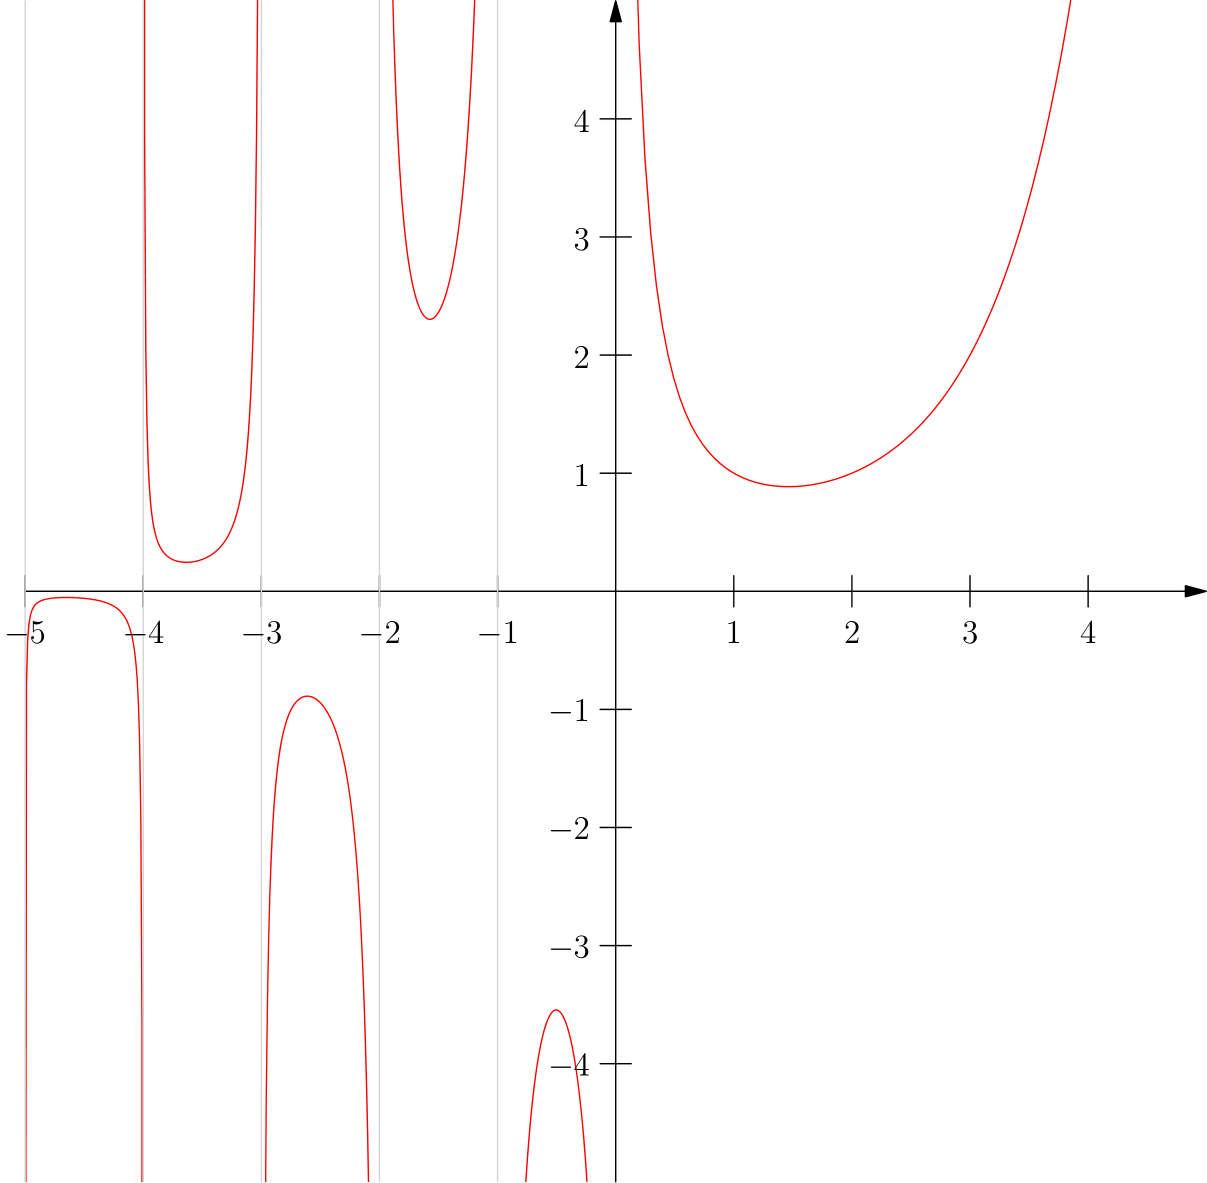
\includegraphics[width=0.5\textwidth]{./figures/gamma_function.png}
    \caption{gamma-function}
    \label{fig:gamma-function}
\end{figure}

% %\begin{figure}
%     %\centering
%     %\begin{tikzpicture}
%         %\begin{axis}[
%             %xmin = -4.9, xmax = 5.1, 
%             %%ymin = -3.5, ymax = 3.5,  
%             %restrict y to domain=-6:6,
%             %axis lines = middle,
%             %axis line style={-latex},  
%             %xlabel={$x$}, 
%             %ylabel={$y$},
%             %%enlarge x limits={upper={val=0.2}},
%             %enlarge y limits=0.05,
%             %x label style={at={(ticklabel* cs:1.00)}, inner sep=5pt, anchor=north},
%             %y label style={at={(ticklabel* cs:1.00)}, inner sep=2pt, anchor=south east},
%             %]
%             %
%             %\addplot[color=red, samples=222, smooth, 
%             %domain = 0:5] gnuplot{gamma(x)};
%             %
%             %\foreach[evaluate={\N=\n-1}] \n in {0,...,-5}{%
%             %\addplot[color=red, samples=555, smooth,  
%             %domain = \n:\N] gnuplot{gamma(x)};
%             %%
%             %\addplot [domain=-6:6, samples=2, densely dashed, thin] (\N, x);
%             %}%
%             %\end{axis}
%     %\end{tikzpicture}
%     %\caption{Гамма-функция}
%     %\label{Гамма-функция}
% %\end{figure}

% %\psset{unit=1.25cm}
% %\begin{pspicture*}(-4.8,-4.8)(4.8,4.8)
% %\psaxes[ticksize=2pt -2pt]{->}(0,0)(-4.8,-4.8)(4.8,4.8)[$ x $, -120][$ y $, -140]
% %\psset{linecolor=Tomato3,linewidth=1.2pt,plotpoints=100,algebraic}
% %\psplot{-4.995}{-4.005}{GAMMA(x)}
% %\psplot{-3.995}{-3.01}{GAMMA(x)}
% %\psplot{-2.99}{-2.05}{GAMMA(x)}
% %\psplot{-1.95}{-1.05}{GAMMA(x)}
% %\psplot{-0.9}{-0.1}{GAMMA(x)}
% %\psplot{.1}{5.8}{GAMMA(x)}
% %\psset{linewidth = 0.6pt, linecolor = LightSteelBlue3}
% %\multido{\i=-4+1}{4}{\psline(\i, -5.8)(\i, 5.8)}
% %\end{pspicture*}

\begin{note} Аналог формулы стрилинга.
     При $p \to \infty $  верно, что $\Gamma (p) = \sqrt {2 \pi p} \left( \dfrac{p}{e} \right) ^p e^{\frac{\Theta}{12}}$, где $\Theta \in (0, 1)$. 
\end{note}

\section{Бета-функция}

\begin{definition}
    $B(p, q) = \int_0^1 x^{p-1}(1-x)^{q-1}dx$

    $B(p, q) = B(q, p) \forall p, q > 0$

    $B(p, q) = \frac{\Gamma(p)\Gamma(q)}{\Gamma(p + q)}$
\end{definition}

\begin{theorem}
    [формула Эйлера-Гаусса]

    \[
    \Gamma(p) = \lim_{k \to \infty} \frac{l^p \cdot k!}{p(p-1) \ldots (p+k)} \quad \forall p\in \R\setminus \Z _-
    .\] 
\end{theorem}

\begin{proof}
    \begin{align*}
        \Gamma(p ) &=\int_0^{+\infty} x ^{p-1} e ^{-x } dx = \Bigg| t = e^{-x}, x = -\ln t, dx = - \dfrac{dt}{t} \Bigg| \int _0^1 (-\ln t)^{p-1} t  \left(- \dfrac{dt}t\right) = \int_{0}^1 (-\ln t)^{p-1)}\\ 
        &= \int_0^1 \left( \lim_{k\to\infty} \underbrace{k (1 - t^{1/k})}_{g(k)}\right)^{p-1} dt ==\\ %
        \p g (k) &= (1 - t^{1/k}) + k (- t^{1/k})\cdot (\ln t) \cdot  \left( + \dfrac{1}{k^2} \right)\\
        &= t^{\frac{1}{k}}\left( t^{- \frac{1}{k}}  - 1 + \frac{\ln t}{k}\right)  \\
        &= \begin{cases}
            f\uparrow&, \text{ если } p\geqslant 1 \implies \text{Применим теорему Леви}\\
            f\downarrow&, \text{ если } p\in (0,1) \implies g(k) \leqslant g(1)\\
        \end{cases} \\
        &== \lim_{k \to \infty} \int_0^1 \left( k(1 - t^{\frac{1}{k}}) \right)^{p-1}dt  = \lim_{k \to \infty} k^{p-1} \int_0^1 s^{p-1} (-k)(1-s)^{k-1}ds = \lim_{k \to \infty} k^p B(p, k) \\
        &= \lim_{k \to \infty} k^p \frac{\Gamma(p)\Gamma(k)}{\Gamma(p+k)} = \lim_{k \to \infty} k^p \cdot (k-1)! \frac{\Gamma(p)}{(p+k-1)(p+k-2)\ldots p \Gamma(p)}\\
        &= \frac{k^pk!}{p(p+1)\ldots (p+k)} \cdot \underbrace{\frac{p+k}{k}}_{\to 1}.
    \end{align*}

    Для $ p<0$ по индукции по $m\quad p \in \left( -(m+1) , -m\right)  $

    Если формула верна для $p+1$, то 
    \begin{align*}
    \Gamma(p) &= \frac{\Gamma(p+1)}{p}  = \frac{1}{p} \lim_{k \to \infty} \frac{k^{p+1}\cdot k!}{(p+1)(p+2) \ldots (p+k+1)}\\
    &=\lim_{k \to \infty} \frac{k^p\cdot k!}{p(p+1) \ldots (p + k)} \cdot \underbrace{\frac{k}{p+k+1}}_{\to 1}
    .\end{align*}
\end{proof}

\begin{lemma}
Пусть $a \in \R$, $f(x) \in C([a, +\infty))$ и $f$ ограничена на $([a, +\infty))$~:~~$\int_a^{+\infty } f(x) dx$ сходится. 
Тогда \[I(y) = \int_a^{+\infty }e^{-xy}f(x)dx \in C([0, +\infty )).\]
\end{lemma}
\begin{proof}
    $A \in [a, +\infty)$

    \begin{align*}
        \int_A^{+\infty }e^{-xy} f(x) dx &= \Bigg| F(x) = \int_A^x f(t)dt \Bigg|  = (F(x) - F(A))\cdot e^{-xy}\mid_A^{+\infty } + \int_A^{+\infty } ye^{-xy} ( F(x) - F(A) ) dx\\
        &= \Bigg| \exists \lim_{x \to \infty} F(x) \left( = \int_A^{+\infty } f(t) dt \right).
    \end{align*}

    Для $\varepsilon >0 \exists A: \left| \int_X^{+\infty }f(t)dt \right| < \frac{\varepsilon}{3}\quad \forall x \geqslant A $

    Для $x \geqslant A\quad \left| F(x) - FA(A) \right|  = \left| \int_X^{+\infty }f(t)dt \right|< \frac{\varepsilon}{3} $
    
    \begin{align*}
    \left| I_A(y) \right| &\leqslant \int_A^{+\infty }ye^{-xy}\left| F(x) - F(A) \right|dx \\
    &< \frac{\varepsilon}{3}\int_0^{+\infty } ye^{-xy}dx = \frac{\varepsilon}{3}\\
    I(y) &= \overbrace{\int_a^Ae^{-xy}f(x)dx}^{J_A(y)} + I_A(y)\\
    I(y) - I(y_0) &= J(y) - J(y_0) + \overbrace{I_A(y) - I_A(y_0)}^{< \frac{\varepsilon}{3}}
    .\end{align*}

    $J(y) - J(y_0) \to 0$ при $y \to y_0$ (условие непрерывности собственных интегралов). 
    \[\exists V(y_0):\quad \forall y\in V(y_0)\, \left| J(y) - J(y_0) \right|< \frac{\varepsilon}{3}. \]
\end{proof}

\begin{corollary}
    \[
    \int_a^{+\infty }f(x)dx = \int_a^{+\infty }\lim_{y \to 0} e^{-xy}f(x)dx.\] 
\end{corollary}

\begin{example}
    [Одно из значений интегрального синуса]
    \begin{align*}
        \int_{0}^{+\infty} \dfrac{\sin x} { x}&\\
        I(y) &= \int_0^\infty \underbrace{e^{-xy } \dfrac{\sin x}{x}}_{f(x,y)} dx\\
        \frac{\partial f}{\partial x} &= -e^{-xy}\sin x\\
        y_0 > 0\quad V_{y_0} &= \left( \frac{y_0}{2}, 2y_0 \right) \implies \left| \frac{\partial f}{\partial y} \right| \leqslant e^{-\frac{xy_0}{2}}\\ 
        \implies \forall y_0& \p I(y) = -\int_0^{+\infty }e^{-xy}\sin x dx\ldots\\
        I(y) &= \int_0^{+\infty} e^{-xy} d cos x = cos x \cdot e^{-xy} \mid_0^{+\infty} + y \int_{0}^{+\infty} \p(\sin x) e^{-xy} dx\\
        &= -1  +  y\left( \sin x e^{-xy} \mid_0^{+\infty} +y \int_{0}^{+\infty} \sin x e ^{-xy} dx \right) = -1 + y^2 \left(-I(y) \right)\\
        \implies& I(y) \cdot(1 + y^2) = -1.\\
        \p I(y) &= I(y) = \left( - \dfrac{1}{1 + y^2}\right) \implies I(y) = C - \int \dfrac{dy}{1+y^2} = C - \arctg y \\
        y\to +\infty, y \geqslant 1& \bigg| e^{-xy} \dfrac{\sin x } {x} \bigg| \leqslant e^{-x}\text{~--- суммируемая мажоранта.}\\
        C - \dfrac{\pi}{2} &= \lim_{y\to \infty} e^{-xy} \dfrac{\sin x} {x} dx = 0 \implies C = \dfrac{\pi}2\\
        I(y)& = \dfrac{\pi}2 - \arctg y \forall y > 0.
    \end{align*}
    Но по лемме $I(y)$ неотрицательная в точке $y = 0$.
    \[ I(0) = \lim_{y \to 0} I(y) = \lim_{y \to 0} \left( \dfrac{\pi}2 - \arctg y \right) =\dfrac{\pi}2 \implies \int_0^{+\infty } \dfrac{\sin  x}x dx = \dfrac{\pi}2. \]
\end{example} %ура, ноль ошибок

\paragraph{Дифференцирование интеграла по параметру в случае переменных пределов интегрирования.}

\[ I(y) = \int_{\alpha(y)}^{\beta(y)} f(x, y) dx;~~~ f \in C \left( [a, b] (x \ni) \times [c, d]  (\ni y)\right),~~~
\alpha(y), \beta(y) : [c, d] \to [a, b] \text{ дифф.} 
\]


\begin{figure}
    \centering
    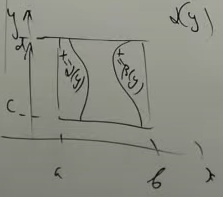
\includegraphics[width=0.3\textwidth]{./img/intergal-with-parametric-bounds.png}
    \caption{Инетграл с переменными пределами}
\end{figure}

\begin{theorem}
    [Правило Лейбница]
Тогда $I(y)$ дифференцируемо на $[c, d]$ и 
\[
    I(y) = \int_{\alpha(y)}^{\beta(y)}\p f_y(x, y)dx + f(\beta(y), y)\cdot \p \beta(y) - f\left( \alpha(y), y \right) \cdot \p\alpha(y)
.\] 
\end{theorem}
\begin{proof}
    \begin{align*}
        \Phi(x, y) &= \int_a^x f(t, y)dt \\ 
        \frac{\partial \Phi}{\partial x} &= f(x, y) \text{ непрерывна в }Q\\
        \frac{\partial \Phi}{\partial y} &= \lim_{\Delta \to y} \frac{1}{\Delta y} \left( \int_a^x f(t, y + \Delta y)dt - \int_a^x f(t,y )dt \right)\\
        &= \int_a^x \p f_y(t, y)dt \\
        \frac{\partial \Phi}{\partial y}(x_1, y_1) - \frac{\partial \Phi}{\partial y}(x, y) = \int_a^x \p f_y(t, y_1)dx  + \left( \int_a^x \p f_y(t, y)dx - \int_a^x \p f_y(t, y)dx \right)  - \int_a^x \p f_y(t, y)dx
    .\end{align*}

    Таким образом $\Phi(x, y)$ дифферецируема на $Q$
    \begin{align*}
        I(y) &= \Phi(\beta(y), y) - \Phi(\alpha(y), y) \\
        \p I(y) = \p Phi_x(\beta(y), y)\cdot \p \beta(y) + \p \Phi_y(\beta(y), y) - \p \Phi_x(\alpha(y), y)\cdot \p \alpha(y) - \p\Phi_y(\alpha(y), y).
    \end{align*}
\end{proof}

\begin{example}
    \[I(p) = \int_{p^2}^{p^3} \dfrac{x^2+ 2p }{\ln^2 |x| + 1} dx \]

    $\forall p \neq 0,\quad [a,b] = [p-\delta, p + \delta]\quad [c,d]$
    \[ \p I(p ) = \int_{p^2}^{p^3} \dfrac{2}{\ln^2 |x| + 1}  dx + \dfrac{p^6 + 2p}{\ln^2 |p^3 | + 1} \cdot 3 p^2 - \dfrac{p^4 + 2p}{\ln^2 |p^2 | + 1} \cdot 2p.\]
\end{example}

\section{Интегрирование на многообразиях}

\begin{definition}
    $\gamma: [a,b] \to \R$ кусочно-гладкое, простой путь (биекция) или заскнутый простой (едиснтвенная точка самопересечния -- концы).

    Пусть $\Gamma = \gamma ([a, b])$~--- носитель нашего пути\dots

    $\mathscr{B} = \{ B~\mid~ \gamma^{-1} (B) \in \mathscr{A}$.
    
    $ds = \nu(B) = \int_{\gamma^{-1}(B)} \|\p \gamma\|(t)dt$.

    $f~:~ \Gamma \to \R(\C)$. $\int_B f ds = \int_{\gamma^{-1} (B) } f (\gamma(t)) \cdot \| \p \gamma (t) \|$.

    Интеграл не зависит от выбора параметризации. Также не зависит от ориентации кривой.
\end{definition}

\begin{example}
    $\int_C x^2sd\qquad C: \begin{cases}
        x^2+y^2+z^2 = R^2\\
         x+y+z = 0\\
    \end{cases}$

    \begin{align*}
        I = \int_C x^2ds = \int_C y^2ds = \int_C z^2ds
        \implies I = \dfrac{1}{3 } \int_C \underbrace{x^2 + y^2 + z^2}_{= R^2} ds = \dfrac{R^2} {3} \int_C ds = \dfrac{R^2} {3} \cdot 2\pi R.
        .\end{align*}
\end{example}

%% нижняя строка, которую можно двигать
\section{Я чуть  чуть опаздал}

\subsection{Многообразие с краем}

\paragraph*{Напоминание}

$k$--мерную $r$--гладкую поверхность в $\R^n$ (многообразие без края).

Пусть $\mathcal M \subseteq \R^n, x^0 \in \mathcal M$.

Окрестность $U_M (x^0) = m \cap U(x^0)$, где $U(x^0)$ --- открытое в $\R^n$.

$\exists ~$ открытое $D \subseteq \R^k$, ~$\Phi : D \to U_M(x^0)$, где
$\Phi \in C^k (D)$, регулярно.

\begin{definition}
    Стандартный куб в $\R^k$ --- это $(-1, 1)^k$.
\end{definition}

\begin{definition}
    Стандартный полукуб в $\R^k$ --- это $[-1, 0] \times (-1, 1)^{k -1}$ при $k > 1$ и $(-1, 0]$ или $[0, 1)$ при $k = 1$.
\end{definition}

\begin{center}
    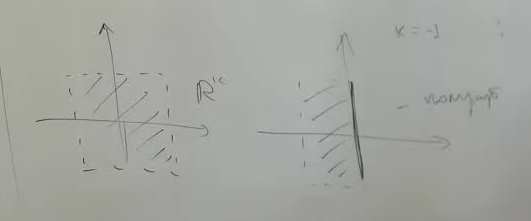
\includegraphics[scale=0.55]{img/simple-squere-and-halfsquere.png}
\end{center}

\begin{definition}
Пусть $\mathcal M \subseteq \R^n$. $\mathcal M$ называется $k$--мерным многообразием с краем, если $\forall x^0 \in \mathcal M \exists $ окрестнось $U_M (x^0)$ и $\Phi ~:~ \Pi_k \to U_M (x^0)$, регулярно и $\in C^k$.

Здесь $\Pi_k$ --- стандартный $k$--мерный куб или стандартный $k$--мерный полукуб.
\end{definition}

$U_M (x^0)$~--- стандартныя окрестнось точки $x^0$  в $\mathcal M$.

$\Phi$~--- локальная параметризация (стандартная).

$\langle U_M(x^0), \Phi\rangle $~--- карта; набор карт~--- атлас.

\begin{example}Очевидные:
    \begin{enumerate}
        \item $(-1, 1)^k$~--- $k$--мерное многообразие (без края).
        \item $(-1, 0] \times (-1, 1)^{k-1}$~--- $k$--мерное многообразие с краем.
        \item $\mathbb{M}_{k, n}^{(r)}$~--- набор $k$--мерных многообразий с краем в $\R^n$ гладкости $r$.
    \end{enumerate}
\end{example}

\begin{center}
    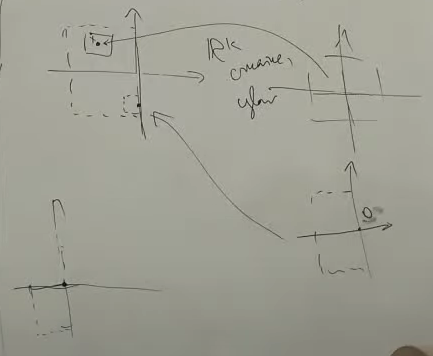
\includegraphics[scale=0.5]{img/k-dimensional-variety-ex1.png}
\end{center}

\begin{example} Чуть менее очевидныей пример.

    $\R^n \in \mathbb{M}_{n,n}^{(\infty)}$~--- многообразие с краем (край пустой).

    \[ \Phi(x_1, \dots, x_n) = \left( \tg \left(x_1 \cdot \dfrac{\pi}{2}\right), \tg \left(x_2 \cdot \dfrac{\pi}{2}\right) \right), \dots, \tg \left(x_n \cdot \dfrac{\pi}{2}\right), ~~~ |x_i| < 1.\]
\end{example}

\begin{definition}
    Пусть $\mathcal M \in \mathbb{M}_{k,n}^{(r)}$.  $x^0 \in \mathcal M$ называется внутренней (относительно многообразия), если $\exists $ стандартная локальная параметризация $\Phi ~:~ \Pi \to U_M(x^0)$, такая, что $\Pi$~--- куб.
\end{definition}

Если точка $x^0$ не является внутренней, то она называется крайней (точкой края).

$\partial \mathcal M = $ множество крайних точек $\mathcal M$ (край $\mathcal M$).

\begin{note}
    Если $\exists$ стандартная параметризация $\Phi ~:~ \Pi \to U_M (x^0)$, такая что $\Pi$~--- полукуб, то $\forall $ стандатной параметризации $\psi ~:~ \tl \Pi \to \tl U_M (x^0)$, $\tl \Pi$~--- полукуб.
\end{note}

\begin{center}
    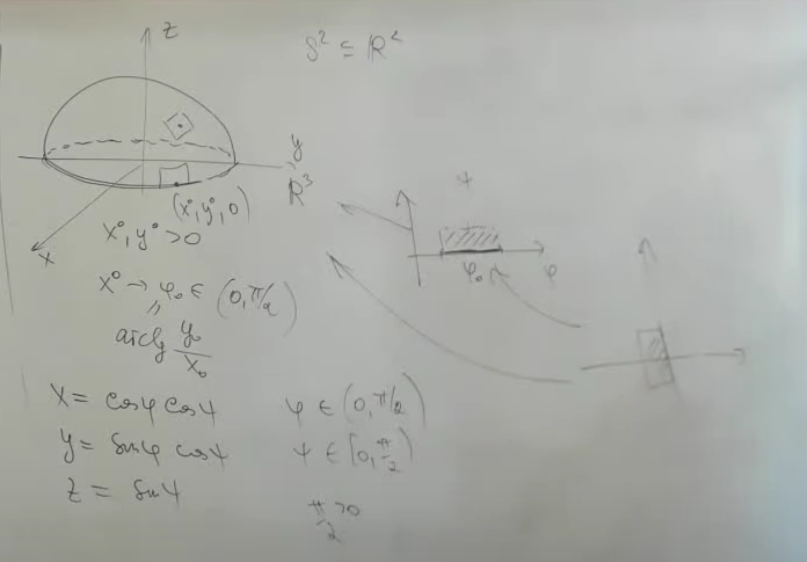
\includegraphics[scale=0.4]{img/halfsphere-to-extreme-points.png}
\end{center}

\begin{note}
    $\mathrm{Fz} \mathcal M \neq \partial \mathcal M$. То есть множество крайних точек не равно множеству граничных точек.
\end{note}

\begin{definition}
    Дискретное множество в $\R^n$ -- множество без предельных точек в $\R^n$

    Само множество не более, чем счётно. В любом шаре $\R^n$ лишь конечное множество точек.

    Дискретное множество в $\R^n$ -- многообразие размерности $0$ в $\R^n$ -- $\mathbb M_{0, n}$
\end{definition}

\begin{example}
    [Конус]

    \[
    ax^2 + by^2 = z^2
    .\]

    В нуле ранг нарушается. Весь конус целиком не многообразие.
\end{example}
% строчк

$\sqsupset  \left( U(x_0), \Phi \right) , \left( \tl U(x_0), \Psi  \right) $ -- две карты для $M in \mathbb M_{k, n}^{(r)},k\in \N $

$V = U(x_0) \cap \tl U(x_0)$

$\Phi^{-1}(C) = W\quad \Psi^{-1}(V) = \tl W$

$\Theta = \Psi^{-1} \circ \Phi\qquad \Theta: W \to \tl W$ -- отображение перехода.

\begin{statement}
    В условия определения отображения перехода оно есть диффеоморфизм из $W$ в $\tl W$.
\end{statement}

\begin{example} Параметризация поверхности сферы через полярные координаты.
    \[ \Phi: (\phi, \psi) \to \begin{bmatrix} \cos\varphi\cos\psi \\ \sin\varphi\cos\psi \\ \sin\psi \end{bmatrix},
    \Psi: (x,y) \to \begin{bmatrix} x \\ y \\ \sqrt{1 - x^2 - y^2}  \end{bmatrix}.\]

    \begin{center}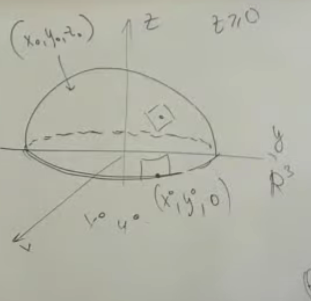
\includegraphics[width=0.25\textwidth]{img/parmetrization-surface-of-sphere.png}
    \end{center}

    \[ \theta: (\varphi, \psi) \to (x,y),~~~
    \theta(\varphi, \psi) = \begin{bmatrix} \cos\varphi\cos\psi \\ \sin\varphi\cos\psi \end{bmatrix},~~~
    \p \theta = \begin{bmatrix}
        -\sin\varphi\cos\psi & -\cos\varphi\sin\psi \\
        \cos\varphi\cos\psi & -\sin\varphi\sin\psi\\
    \end{bmatrix}. \]

    $\det \p \theta = \cos\pi\sin\psi$

    $\pi_{x_1, \ldots, x_k}\Psi : \Pi\in \R^n \to \R^k$ -- локально диффеоморфизм

    $(g = \pi \circ \psi)^{-1}: (x_1, \ldots, x_k) \to (v_1, \ldots, v_k)\qquad x_{k+1}, \ldots, x_n$ -- функции от первых координат

    $\Theta = g \circ \pi_{x_1, \ldots, x_k}\Phi$. Аналогично устроено обратное отображение, значит определители обоих не могут обращаться в ноль.
\end{example}

\begin{corollary}
    Инвариантность типа множества (куб или полукуб) от выбора станратной параметриазации вытекает из последнего утверждения,
\end{corollary}

\begin{corollary}
    $\forall \mathcal M \in \mathbb M_{k,n}^{(r)}\quad \forall x^0\in \mathcal M$ лькально некоторые $n-k$ координат точки выражаются как функции от остальных координат.
\end{corollary}

\begin{note}
  Касательное пространство -- пространство касательных векторов (векторов принадлежащих какой-то кривой на поверхности).

    $\Tp \mathcal M = d_{\Phi^1(p)}\Phi(\R^k)$
\end{note}

\begin{definition}
    $\sqsupset \mathcal M \in \mathbb M_{k, n}^{(1)}\quad x^0\in \mathcal M\quad (U(x_0), \Phi)$ -- карта

    $T_{x_0}\mathcal M = d_0\Phi(\R^k)$
\end{definition}

\begin{note}
    Определение $T_{x^0}\mathcal M$ не зависит от параметризации.
    \[
    d_0\Phi(\R^k) = d_0(\Psi_0\theta)(\R^k) = f_{\theta(0)}\Psi(d_0\theta (\R^k))  = d_{\theta(0) = 0}\Psi(\R^k)
    .\]

    $d_0\theta$ -- изоморфизм, т.к. $\theta$ -- диффеоморфизм.
\end{note}

\begin{note}
    $N \in \R, N$ -- нормальный вектор к $\mathcal M$  в точке $x^0$, если $N \perp T_{x^0}\mathcal M$. (Иногда требуют длину 1, но часто нет)
\end{note}
\begin{note}
    Если $M\in \mathbb M_{k,n}^r$ в окрестности $x^0$ задаётся системой $\begin{cases}
        F_1(x) = 0\\
        \ldots\\
        F_{n-k}(x) = 0\\
    \end{cases}$

    $\nabla F_1, \ldots, \nabla F_{n-k}$ -- базис $(T_{x^0} \mathcal M)^{\perp}$

\end{note}

\begin{note}
    Если $\mathcal M\in M_{n-1,n}^{(1)}\quad N \perp T_{x^0}\mathcal M\quad N = \left|
        \begin{matrix}
            e_1& e_2& \ldots& e_n\\
            && \frac{\partial \Phi}{\partial u_1}(0)&\\
            && \vdots&\\
            && \frac{\partial \Phi}{\partial u_n}(0)&\\
        \end{matrix}
    \right| $

    $(U(x_0), \Phi)$ -- карта

    $\iff N \perp \frac{\partial \Phi}{\partial u_j}(0)\quad \forall j = 1, \ldots, n-1$

    $\left<N, \frac{\partial \Phi}{\partial u_j}(0) \right> = \left|
        \begin{matrix}
            && \frac{\partial \Phi}{\partial u_j}(0)&\\
            && \frac{\partial \Phi}{\partial u_1}(0)&\\
            && \vdots&\\
            && \frac{\partial \Phi}{\partial u_n}(0)&\\
        \end{matrix}
    \right| = 0 $, т.к. совпадают две строки.

    Частный случай. Пусть $n = 3$, $k = 2$. $\mathcal M$~--- график $z = g(x, y)$, заданный на открытом множестве $D \subseteq \R^2$, $g \in C^1$.

    \[ \Phi :(x, y) \to (x, y, z) = (x, y, g(x, y)),~~~
     \p \Phi = \begin{pmatrix}
        1 & 0 \\ 0 & 1 \\ \p g_x & \p g_y
    \end{pmatrix}\]

    Таким образом, $\mathcal{M}$~--- двумерное многообразе хотя бы класса $C^{(1)}$, то есть $\mathcal M \in \mathbb M_{2, 3}^{(1)}$.

    $N$~--- нормаль к $\mathcal{M}$, ~$N = \begin{bmatrix}
        \vec{i}& \vec{j} & \vec{k} \\ 1 & 0 & \p g_x \\ 0 & 1 & \p g_y
    \end{bmatrix} = \left( -\p g_x , -p g_y, 1 \right)$~--- направлена вверх.
\end{note}

\begin{definition}
    $\sqsupset (U(x^0), \Phi), (\tl U(x^0), \Psi)$ -- две карты

    $x_0\in \mathcal M\quad \mathcal M\in \mathbb M_{k, n}^{(r)}$

    Скажем, что $\Phi$ и $\Psi$ согласованы, если $\det \Theta >0$, где $\theta = \Psi^{-1}\circ\Phi$ -- отображение перехода.
\end{definition}

\begin{note}
    Отношение согласованности является отношение эквивалентности.
    % Отображение перехода образует отношение эквивалентности.
\end{note}

\begin{definition}
    $I(x^0)$ называется ориентированной, если зафиксирован один из классов экивалентности по отношению согласованности.
\end{definition}

\begin{note}
    $\sqsupset U(x^0) \cap U(x^1) \neq 0$. $U(x^0)$ И $U(x^1)$  согласованы, если $\Phi\in U_+(x^0), \Psi\in U_+(x^1)$, где $U_+$ -- зафиксирванный класс.
    $ \implies \det(\Psi^{-1}\circ\Phi) >0$

    Если $U(x^0) \cap U(x^1) = \O $, то их ориентации согласованы.

    Атлас $A = \{(U, \Phi)\}$ многообразия $\mathcal M$ называется ориентированным, если ориентации любых двух $U, V\in A$ согласованы.

    Многообразие с краем называется ориентиркемым, если $\exists $ ориентированный атлас.
\end{note}

\begin{definition}
    Пусть $\Gamma = \mathcal{M} \in \mathbb{M}_{1, n}^{(1)}$, ~ $\tau ~:~ \mathcal M \to \R^n$ и $\forall x^0 \in \mathcal{M}~:~ \tau (x^0) \in T_{x^0} \circ \mathcal M$, ~$\tau$~--- непрерывное, $\|\tau\| \equiv 1$.

    Тогда $\tau$ называется направлением на $\mathcal M$.
\end{definition}


\begin{statement}
    $\forall $ связное $1$--менрное, $1$--глакое многообразе с краем имеет ровно два направления.

    $ \tau (x) =  \pm \dfrac{\p \gamma}{\| \p \gamma \|} ~~(\gamma ^{-1} (x))$, где $\gamma$~--- параметризация из выбранного класса эквивалентности (из ориентации окрестности $\mathcal{M}$).
\end{statement}

\begin{definition}
    $k = n-1\quad n\in \N , n\geqslant 2\quad \mathcal M \in \mathbb M_{n-1, n}^{(\perp)}$

    $n(x) : \mathcal M \to \R^n$ называется стороной, если:
    \begin{enumerate}
        \item $n(x)\in C(M)$
        \item $\forall x\in \mathcal M\quad n(x)\perp T_x \mathcal M$
        \item $\|n(x)\| = 1$
    \end{enumerate}
\end{definition}

\begin{note}
    Сторон чётное число.
\end{note}

\begin{note}
    Не у всех поверхностей есть сторона. Лента Мёбиуса, бутылка Клейна, \ldots

    \begin{center}
        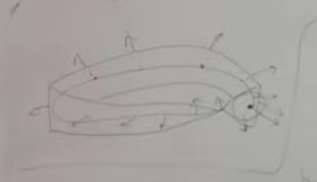
\includegraphics[scale=0.5]{img/moebius-tape.png}
    \end{center}
\end{note}

\begin{statement}
    Для $k = n-1$ ориентируемость многообразия с краем $\mathcal M \in (\mathbb M_{n-1, n}^1)$ равносильно существоавнию стороны.
\end{statement}

\begin{theorem}
    Пусть $\mathcal M\in \mathbb M^{(1)}_{k, n}\quad K\leqslant n, k, n\in \N $

    Тогда:
    \begin{enumerate}
        \item $\partial \mathcal {M} \in \mathbb{M}_{k-1 ,n}^{(1)}$; $\partial \left(\partial \mathcal{M}\right) = \varnothing $
        \item Если $\mathcal M$ -- ориентированно то $\partial \mathcal M$ ориентируем.
    \end{enumerate}
\end{theorem}
\begin{proof}
    $\partial \mathcal M$ -- многообразие без края.
\end{proof}

\begin{center}
    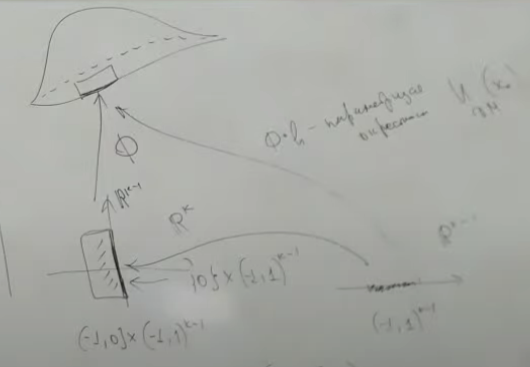
\includegraphics[scale=0.4]{img/extreme-points-of-extreme-points-ex1}
\end{center}

%%%
\section{Я чуть  чуть опаздал}

\subsection{Многообразие с краем}

\paragraph*{Напоминание}

$k$--мерную $r$--гладкую поверхность в $\R^n$ (многообразие без края).

Пусть $\mathcal M \subseteq \R^n, x^0 \in \mathcal M$.

Окрестность $U_M (x^0) = m \cap U(x^0)$, где $U(x^0)$ --- открытое в $\R^n$.

$\exists ~$ открытое $D \subseteq \R^k$, ~$\Phi : D \to U_M(x^0)$, где
$\Phi \in C^k (D)$, регулярно.

\begin{definition}
    Стандартный куб в $\R^k$ --- это $(-1, 1)^k$.
\end{definition}

\begin{definition}
    Стандартный полукуб в $\R^k$ --- это $[-1, 0] \times (-1, 1)^{k -1}$ при $k > 1$ и $(-1, 0]$ или $[0, 1)$ при $k = 1$.
\end{definition}

\begin{center}
    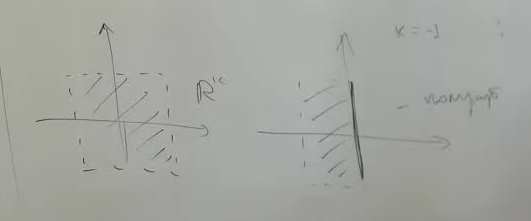
\includegraphics[scale=0.55]{img/simple-squere-and-halfsquere.png}
\end{center}

\begin{definition}
Пусть $\mathcal M \subseteq \R^n$. $\mathcal M$ называется $k$--мерным многообразием с краем, если $\forall x^0 \in \mathcal M \exists $ окрестнось $U_M (x^0)$ и $\Phi ~:~ \Pi_k \to U_M (x^0)$, регулярно и $\in C^k$.

Здесь $\Pi_k$ --- стандартный $k$--мерный куб или стандартный $k$--мерный полукуб.
\end{definition}

$U_M (x^0)$~--- стандартныя окрестнось точки $x^0$  в $\mathcal M$.

$\Phi$~--- локальная параметризация (стандартная).

$\langle U_M(x^0), \Phi\rangle $~--- карта; набор карт~--- атлас.

\begin{example}Очевидные:
    \begin{enumerate}
        \item $(-1, 1)^k$~--- $k$--мерное многообразие (без края).
        \item $(-1, 0] \times (-1, 1)^{k-1}$~--- $k$--мерное многообразие с краем.
        \item $\mathbb{M}_{k, n}^{(r)}$~--- набор $k$--мерных многообразий с краем в $\R^n$ гладкости $r$.
    \end{enumerate}
\end{example}

\begin{center}
    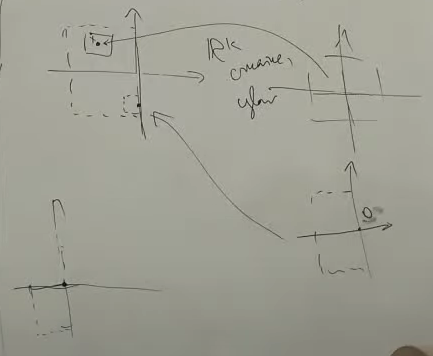
\includegraphics[scale=0.5]{img/k-dimensional-variety-ex1.png}
\end{center}

\begin{example} Чуть менее очевидныей пример.

    $\R^n \in \mathbb{M}_{n,n}^{(\infty)}$~--- многообразие с краем (край пустой).

    \[ \Phi(x_1, \dots, x_n) = \left( \tg \left(x_1 \cdot \dfrac{\pi}{2}\right), \tg \left(x_2 \cdot \dfrac{\pi}{2}\right) \right), \dots, \tg \left(x_n \cdot \dfrac{\pi}{2}\right), ~~~ |x_i| < 1.\]
\end{example}

\begin{definition}
    Пусть $\mathcal M \in \mathbb{M}_{k,n}^{(r)}$.  $x^0 \in \mathcal M$ называется внутренней (относительно многообразия), если $\exists $ стандартная локальная параметризация $\Phi ~:~ \Pi \to U_M(x^0)$, такая, что $\Pi$~--- куб.
\end{definition}

Если точка $x^0$ не является внутренней, то она называется крайней (точкой края).

$\partial \mathcal M = $ множество крайних точек $\mathcal M$ (край $\mathcal M$).

\begin{note}
    Если $\exists$ стандартная параметризация $\Phi ~:~ \Pi \to U_M (x^0)$, такая что $\Pi$~--- полукуб, то $\forall $ стандатной параметризации $\psi ~:~ \tl \Pi \to \tl U_M (x^0)$, $\tl \Pi$~--- полукуб.
\end{note}

\begin{center}
    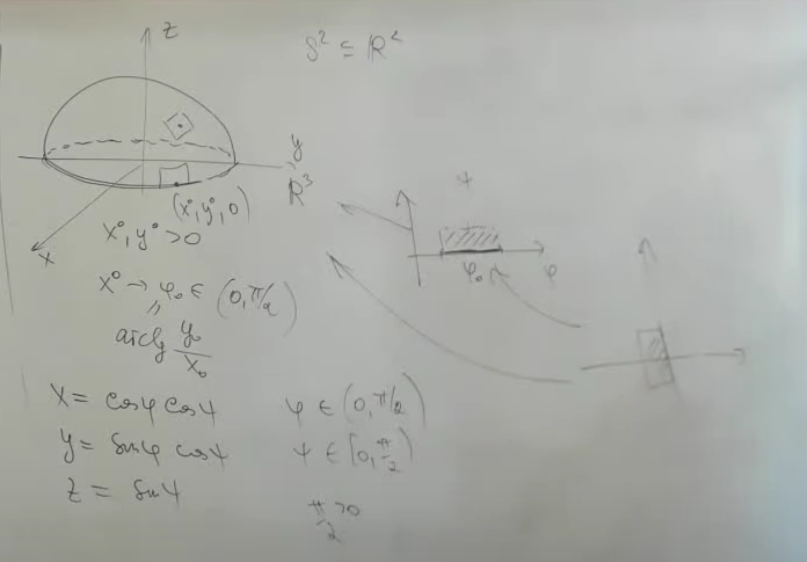
\includegraphics[scale=0.4]{img/halfsphere-to-extreme-points.png}
\end{center}

\begin{note}
    $\mathrm{Fz} \mathcal M \neq \partial \mathcal M$. То есть множество крайних точек не равно множеству граничных точек.
\end{note}

\begin{definition}
    Дискретное множество в $\R^n$ -- множество без предельных точек в $\R^n$

    Само множество не более, чем счётно. В любом шаре $\R^n$ лишь конечное множество точек.

    Дискретное множество в $\R^n$ -- многообразие размерности $0$ в $\R^n$ -- $\mathbb M_{0, n}$
\end{definition}

\begin{example}
    [Конус]

    \[
    ax^2 + by^2 = z^2
    .\]

    В нуле ранг нарушается. Весь конус целиком не многообразие.
\end{example}
% строчк

$\sqsupset  \left( U(x_0), \Phi \right) , \left( \tl U(x_0), \Psi  \right) $ -- две карты для $M in \mathbb M_{k, n}^{(r)},k\in \N $

$V = U(x_0) \cap \tl U(x_0)$

$\Phi^{-1}(C) = W\quad \Psi^{-1}(V) = \tl W$

$\Theta = \Psi^{-1} \circ \Phi\qquad \Theta: W \to \tl W$ -- отображение перехода.

\begin{statement}
    В условия определения отображения перехода оно есть диффеоморфизм из $W$ в $\tl W$.
\end{statement}

\begin{example} Параметризация поверхности сферы через полярные координаты.
    \[ \Phi: (\phi, \psi) \to \begin{bmatrix} \cos\varphi\cos\psi \\ \sin\varphi\cos\psi \\ \sin\psi \end{bmatrix},
    \Psi: (x,y) \to \begin{bmatrix} x \\ y \\ \sqrt{1 - x^2 - y^2}  \end{bmatrix}.\]

    \begin{center}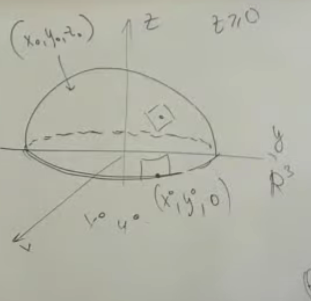
\includegraphics[width=0.25\textwidth]{img/parmetrization-surface-of-sphere.png}
    \end{center}

    \[ \theta: (\varphi, \psi) \to (x,y),~~~
    \theta(\varphi, \psi) = \begin{bmatrix} \cos\varphi\cos\psi \\ \sin\varphi\cos\psi \end{bmatrix},~~~
    \p \theta = \begin{bmatrix}
        -\sin\varphi\cos\psi & -\cos\varphi\sin\psi \\
        \cos\varphi\cos\psi & -\sin\varphi\sin\psi\\
    \end{bmatrix}. \]

    $\det \p \theta = \cos\pi\sin\psi$

    $\pi_{x_1, \ldots, x_k}\Psi : \Pi\in \R^n \to \R^k$ -- локально диффеоморфизм

    $(g = \pi \circ \psi)^{-1}: (x_1, \ldots, x_k) \to (v_1, \ldots, v_k)\qquad x_{k+1}, \ldots, x_n$ -- функции от первых координат

    $\Theta = g \circ \pi_{x_1, \ldots, x_k}\Phi$. Аналогично устроено обратное отображение, значит определители обоих не могут обращаться в ноль.
\end{example}

\begin{corollary}
    Инвариантность типа множества (куб или полукуб) от выбора станратной параметриазации вытекает из последнего утверждения,
\end{corollary}

\begin{corollary}
    $\forall \mathcal M \in \mathbb M_{k,n}^{(r)}\quad \forall x^0\in \mathcal M$ лькально некоторые $n-k$ координат точки выражаются как функции от остальных координат.
\end{corollary}

\begin{note}
  Касательное пространство -- пространство касательных векторов (векторов принадлежащих какой-то кривой на поверхности).

    $\Tp \mathcal M = d_{\Phi^1(p)}\Phi(\R^k)$
\end{note}

\begin{definition}
    $\sqsupset \mathcal M \in \mathbb M_{k, n}^{(1)}\quad x^0\in \mathcal M\quad (U(x_0), \Phi)$ -- карта

    $T_{x_0}\mathcal M = d_0\Phi(\R^k)$
\end{definition}

\begin{note}
    Определение $T_{x^0}\mathcal M$ не зависит от параметризации.
    \[
    d_0\Phi(\R^k) = d_0(\Psi_0\theta)(\R^k) = f_{\theta(0)}\Psi(d_0\theta (\R^k))  = d_{\theta(0) = 0}\Psi(\R^k)
    .\]

    $d_0\theta$ -- изоморфизм, т.к. $\theta$ -- диффеоморфизм.
\end{note}

\begin{note}
    $N \in \R, N$ -- нормальный вектор к $\mathcal M$  в точке $x^0$, если $N \perp T_{x^0}\mathcal M$. (Иногда требуют длину 1, но часто нет)
\end{note}
\begin{note}
    Если $M\in \mathbb M_{k,n}^r$ в окрестности $x^0$ задаётся системой $\begin{cases}
        F_1(x) = 0\\
        \ldots\\
        F_{n-k}(x) = 0\\
    \end{cases}$

    $\nabla F_1, \ldots, \nabla F_{n-k}$ -- базис $(T_{x^0} \mathcal M)^{\perp}$

\end{note}

\begin{note}
    Если $\mathcal M\in M_{n-1,n}^{(1)}\quad N \perp T_{x^0}\mathcal M\quad N = \left|
        \begin{matrix}
            e_1& e_2& \ldots& e_n\\
            && \frac{\partial \Phi}{\partial u_1}(0)&\\
            && \vdots&\\
            && \frac{\partial \Phi}{\partial u_n}(0)&\\
        \end{matrix}
    \right| $

    $(U(x_0), \Phi)$ -- карта

    $\iff N \perp \frac{\partial \Phi}{\partial u_j}(0)\quad \forall j = 1, \ldots, n-1$

    $\left<N, \frac{\partial \Phi}{\partial u_j}(0) \right> = \left|
        \begin{matrix}
            && \frac{\partial \Phi}{\partial u_j}(0)&\\
            && \frac{\partial \Phi}{\partial u_1}(0)&\\
            && \vdots&\\
            && \frac{\partial \Phi}{\partial u_n}(0)&\\
        \end{matrix}
    \right| = 0 $, т.к. совпадают две строки.

    Частный случай. Пусть $n = 3$, $k = 2$. $\mathcal M$~--- график $z = g(x, y)$, заданный на открытом множестве $D \subseteq \R^2$, $g \in C^1$.

    \[ \Phi :(x, y) \to (x, y, z) = (x, y, g(x, y)),~~~
     \p \Phi = \begin{pmatrix}
        1 & 0 \\ 0 & 1 \\ \p g_x & \p g_y
    \end{pmatrix}\]

    Таким образом, $\mathcal{M}$~--- двумерное многообразе хотя бы класса $C^{(1)}$, то есть $\mathcal M \in \mathbb M_{2, 3}^{(1)}$.

    $N$~--- нормаль к $\mathcal{M}$, ~$N = \begin{bmatrix}
        \vec{i}& \vec{j} & \vec{k} \\ 1 & 0 & \p g_x \\ 0 & 1 & \p g_y
    \end{bmatrix} = \left( -\p g_x , -p g_y, 1 \right)$~--- направлена вверх.
\end{note}

\begin{definition}
    $\sqsupset (U(x^0), \Phi), (\tl U(x^0), \Psi)$ -- две карты

    $x_0\in \mathcal M\quad \mathcal M\in \mathbb M_{k, n}^{(r)}$

    Скажем, что $\Phi$ и $\Psi$ согласованы, если $\det \Theta >0$, где $\theta = \Psi^{-1}\circ\Phi$ -- отображение перехода.
\end{definition}

\begin{note}
    Отношение согласованности является отношение эквивалентности.
    % Отображение перехода образует отношение эквивалентности.
\end{note}

\begin{definition}
    $I(x^0)$ называется ориентированной, если зафиксирован один из классов экивалентности по отношению согласованности.
\end{definition}

\begin{note}
    $\sqsupset U(x^0) \cap U(x^1) \neq 0$. $U(x^0)$ И $U(x^1)$  согласованы, если $\Phi\in U_+(x^0), \Psi\in U_+(x^1)$, где $U_+$ -- зафиксирванный класс.
    $ \implies \det(\Psi^{-1}\circ\Phi) >0$

    Если $U(x^0) \cap U(x^1) = \O $, то их ориентации согласованы.

    Атлас $A = \{(U, \Phi)\}$ многообразия $\mathcal M$ называется ориентированным, если ориентации любых двух $U, V\in A$ согласованы.

    Многообразие с краем называется ориентиркемым, если $\exists $ ориентированный атлас.
\end{note}

\begin{definition}
    Пусть $\Gamma = \mathcal{M} \in \mathbb{M}_{1, n}^{(1)}$, ~ $\tau ~:~ \mathcal M \to \R^n$ и $\forall x^0 \in \mathcal{M}~:~ \tau (x^0) \in T_{x^0} \circ \mathcal M$, ~$\tau$~--- непрерывное, $\|\tau\| \equiv 1$.

    Тогда $\tau$ называется направлением на $\mathcal M$.
\end{definition}


\begin{statement}
    $\forall $ связное $1$--менрное, $1$--глакое многообразе с краем имеет ровно два направления.

    $ \tau (x) =  \pm \dfrac{\p \gamma}{\| \p \gamma \|} ~~(\gamma ^{-1} (x))$, где $\gamma$~--- параметризация из выбранного класса эквивалентности (из ориентации окрестности $\mathcal{M}$).
\end{statement}

\begin{definition}
    $k = n-1\quad n\in \N , n\geqslant 2\quad \mathcal M \in \mathbb M_{n-1, n}^{(\perp)}$

    $n(x) : \mathcal M \to \R^n$ называется стороной, если:
    \begin{enumerate}
        \item $n(x)\in C(M)$
        \item $\forall x\in \mathcal M\quad n(x)\perp T_x \mathcal M$
        \item $\|n(x)\| = 1$
    \end{enumerate}
\end{definition}

\begin{note}
    Сторон чётное число.
\end{note}

\begin{note}
    Не у всех поверхностей есть сторона. Лента Мёбиуса, бутылка Клейна, \ldots

    \begin{center}
        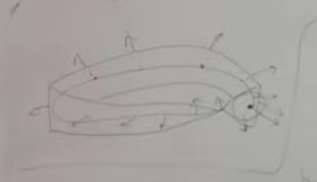
\includegraphics[scale=0.5]{img/moebius-tape.png}
    \end{center}
\end{note}

\begin{statement}
    Для $k = n-1$ ориентируемость многообразия с краем $\mathcal M \in (\mathbb M_{n-1, n}^1)$ равносильно существоавнию стороны.
\end{statement}

\begin{theorem}
    Пусть $\mathcal M\in \mathbb M^{(1)}_{k, n}\quad K\leqslant n, k, n\in \N $

    Тогда:
    \begin{enumerate}
        \item $\partial \mathcal {M} \in \mathbb{M}_{k-1 ,n}^{(1)}$; $\partial \left(\partial \mathcal{M}\right) = \varnothing $
        \item Если $\mathcal M$ -- ориентированно то $\partial \mathcal M$ ориентируем.
    \end{enumerate}
\end{theorem}
\begin{proof}
    $\partial \mathcal M$ -- многообразие без края.
\end{proof}

\begin{center}
    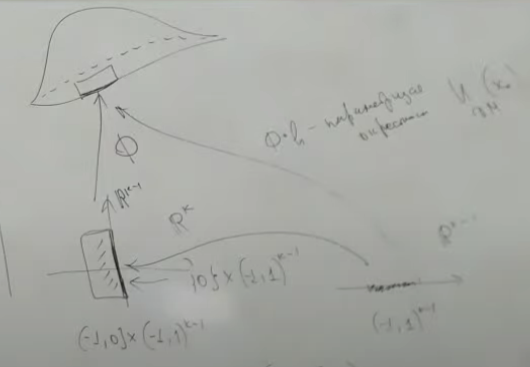
\includegraphics[scale=0.4]{img/extreme-points-of-extreme-points-ex1}
\end{center}

%%%
\begin{note}[Воспоминания]
    Многообразие -- локально гомеоморфно кубу.

    С краем -- есть точки геомеоморфные половине куба.

    Пусть у нас есть две параметризации окрестности: $\Phi, \Psi. \Phi = \Psi \circ \Theta\qquad \Phi \sim \Psi \iff \det \p \Theta > 0$

    Класс эквивалентности $\left[ \Phi \right] $ -- ориентация окрестности

    $U, V$ -- окрестности в  $M$. Они согласованы если:
     \begin{itemize}
        \item они не перескекаются
        \item они пересекаются и $\det \p \theta > 0$, где $\theta$ -- отображение перехода от  $\Phi$ к  $\Psi$, где  $\Phi$ -- из ориентации  $U$,  $\Psi$ -- из ориентации  $V$ и  $\Phi(\Pi) \cap \Psi(\Pi) \neq \O $        
    \end{itemize}
\end{note}

\begin{example}
    $S_1 = S \cap \left\{ z>0 \right\} \quad S_2 = S \cap  \left\{ x>0 \right\} $

    $\theta: (x,y) \to (y, \sqrt{1 - x^2-y^2} $ 

    $\p \theta = \begin{bmatrix} 0&1\\ -\frac{x}{\sqrt{1-x^2-y^2} }& -\frac{y}{\sqrt{1 - x^2-y^2} } \end{bmatrix} $

    $\p \det = \frac{x}{\sqrt{1 - x^2-y^2} }>0$ на области определения ($\Phi^{-1}(S_1\cap S_2)$ )

    $S_3 = S \cap \left\{ z<0 \right\} \quad $

    $\tl \theta(x,y) = (y, -\sqrt{1-x^2-y^2} $ 

    И здесь уже всё плохо с определиителем.
\end{example}

\begin{statement}
    $\sqsupset \gamma: \left<a,b \right>\subseteq \R \to \R^n $, регулярно ($\iff  \p \gamma(t) \neq 0\quad \forall t\in \left<a,b \right>$). $\gamma$ -- простой путь (без самопересечений, инъективность)

    $\Gamma = \gamma\left( \left<a,b \right> \right) $ -- Одномерное многообразие.

    Край не пуст, если $\left\{ a,b \right\} \cap \left<a,b \right>\neq \O $

    Направление -- непрерывное отображение $\tau:\Gamma \to \R^n$:
    \begin{enumerate}
        \item непрерывно $\tau\in C(\Gamma)$
        \item  $\tau(x) \in T_x\Gamma \forall x\in \Gamma$
        \item $\|\tau(x)\| = 1 \forall x\in \Gamma$
    \end{enumerate}

    Для любой гладкой кривой $\Gamma$ (из определения выше) существует ровно два направления на этой кривой, и любая такая  $\Gamma$ ориентируема
\end{statement}
\begin{proof}
    Ориентация порождается сужениями одного и того же отображения $\lambda$ на различные кубы и полукубы.

    \[
        \tau_\gamma = \frac{\p \gamma}{\|\p \gamma\|}\left( \gamma^{-1}(x) \right) 
    .\] 
    $\tau(x)$ -- ещё одно направление

    $t\in \left( a,b \right) \quad h(t) = \left<\tau_\gamma\left( \gamma(t) \right) , \tau(\gamma(t)) \right> = \pm \|\tau_\gamma\left( \gamma(t) \right) \| \|\tau\left( \gamma(t) \right) \| = \pm 1 $

    $h: \left<a,b \right> \to \left\{ -1,+1 \right\} $ -- непрерывно, но $h(\left<a,b \right>)$ должно быть промежутком:
    \begin{enumerate}
        \item $h\left( \left<a,b \right> \right)  = \left\{ 1 \right\} \implies \tau = \tau_\gamma$
        \item $h\left( \left<a,b \right> \right)  = \left\{ -1 \right\} \implies \tau = -\tau_\gamma$
    \end{enumerate}
\end{proof}

\begin{statement}
    $k = n-1\geqslant 2, n\in \N$

    Сторона на многообразии $M\in \mathds M_{n-1, n}^1$ -- отображение  $N: M \to \R^n$:
    \begin{enumerate}
        \item $n\in C\left( M \right) $
        \item $N(x) \perp T_x M$ 
        \item $\|N\| = 1$
    \end{enumerate}

    Если $M\in \mathds M_{n-1, n}^1$. Тогда $M$ двусторонняя $\iff M$ ориентируема. Если $M$ двустороняя, то любая сторона представима в виде:
    \[
        N = \pm\frac{N_{\Phi}}{\|N_\Phi\|}\left( \varphi^{-1}(x) \right) 
    .\] 
    $\Phi$ -- параметризация окрестности точки  $x$ Из выбранной ориентации  

    $N_\Phi = 
    \begin{vmatrix}
        \vec e_1 & \ldots & \vec e_n\\
        \ldots & \p \Phi_{u_1} & \ldots\\
        \ldots& \vdots & \ldots\\
        \ldots & \p \Phi_{u_{n-1}}& \ldots
    \end{vmatrix}$

    $\|N_{\Phi}\| \neq 0$

    $\Phi \sim \tl \Phi$


    
\end{statement}

\begin{note}
    [Напоминание]

    $\mathcal E_p(X)$ -- набор кососимметрических $p$ форм из $X$ в $\R^n$

    $\omega: O \to \mathcal E_p(\R^n)$

    $\omega(x, h^1, \ldots, h^p)\quad h_i\in \R^n$

    $\omega = \sum_{1\leqslant i_1 < i_2 < \ldots < i_p \leqslant n}\omega_{i_1\ldots i_p}dx_{i_1}(x) \wedge \ldots \wedge dx_{i_p} = \sum_I \omega_I(x)dx^I$

    $\Omega_p^{(r)} = \Omega_{p,n}^{(r)}$ -- набор всех дифференцируемых $p$-форм гладкости $r$ в $O$
\end{note}

\begin{example}
    \begin{enumerate}
        \item $f\in C^k(O),\quad \omega = f\in \Omega_0^{(k)}(O)$
        \item $f \in C^k(O),\quad d_xf = \sum_{i=1}^n \frac{\partial f}{\partial x_i}(x)dx_i\in \Omega_1^{(k-1)}(O)$
        \item $\sqsupset F$ -- поле в $\R^3\quad F = (P,Q,R):O \to \R^3$
        $\omega_F = Pdx + Qdy + Rfz$

        $\omega_F(h\in \R^3) = P(x,y,z) h_1 + Q(x,y,z)h^2 + R(x,y,z)h^3$

        Если $h \approx 0 \implies \omega_F(h)\approx$ элементарная работа поля $F$ на перемещение $h$ 

        $\omega_F^* = Pdy\wedge dz + Qdz\wedge dx + Rdx\wedge dy$

        $dy\wedge dz \ldots$ -- задают базис $\Omega_{2,3}$

        $\Omega_1^n $ изоморфно $\Omega_{n-1}^n$
        \item $V = (P,Q,R) \in C^r(O)$ 
        
        $\omega(x,h^1,h^2) = \begin{vmatrix}
            v\\h^1\\h^2
        \end{vmatrix}\in \Omega_{2,3}^{(r)}(O),\quad h61,h^2\in \R^3$ -- смешанное произведение $(h^1,h^2,v)$

        Смысл: Если $V$ -- поле скоростей, а $h^1, h^2\approx 0$, то $\left( h^1,h^2,v \right) $ -- поток поля $V$ через площадку, натянутую на $h^1$ и $h^2$
        
        $\omega = p \begin{vmatrix}
            h_2^1 & h_3^1\\h_2^2 & h_3^2
        \end{vmatrix} + Q \begin{vmatrix}
            h_3^1 & h_1^1\\h_3^2 & h_1^2
        \end{vmatrix} + R \begin{vmatrix}
            h_1^1 & h_2^1\\
            h_1^2 & h_2^2
        \end{vmatrix}$

        $\omega = Pdy\wedge dz + Qdz\wedge dx + Rdx\wedge dy = \omega^*_V$
    \end{enumerate}
\end{example}

\section{Внешнее дифференцирование дифференциальных форм}

``$d$'' --- внещний дифференциал

\begin{definition}
[Внешний дифференцал для форм]
    $\omega  \in \Omega^{(1)}_{0, n} (O)$,~~~ $d_x \omega = \sum_{i=1}^n \dfrac{\partial \omega}{\partial x_i} (x) d x_i$ 


    $\omega \in \Omega_p^(1)(O)\quad \omega = \sum_I \omega_Idx^I, \omega_I\in \Omega_0^{(1)}(O) \implies dw = \sum _I (d\omega_I)\wedge dx^I$
    
    $d\omega \in \Omega_{p+1}^{(0)}(O)\quad dw = \sum_{k=1}^{n} \sum_I \frac{\omega_I}{\partial x_i} dx_i\wedge dx^I$
\end{definition}

\begin{example}
    \begin{enumerate}
        \item $\omega  \in \Omega_{n-1, n}^{(r)} (O)$.
        
        Для $n = 3$:
        $\omega = P dy \wedge dz + Q dz \wedge dx + R dx \wedge dy$.
        
        $d\omega = dP \wedge dy \wedge dz + Q \wedge dz \wedge dx + R \wedge dx \wedge dy = \p P_x dx \wedge dy \wedge dz + \p Q_y dy \wedge dz \wedge dx + \p R_z dz \wedge dx \wedge dy = $\\
        $ \left( \p P_x + \p Q_y + \p R_z \right) dx dy dz \implies d\omega = \mathrm{div} (P, Q, R) dx \wedge dy \wedge dz$.


    
        $d\omega = \div(P,Q,R)\cdot dx\wedge dy\wedge dz = d \omega_{(P, Q, R)}^{*}$.

        $\omega = Pdx + Qdy + Rdz$

        $d\omega = \left( \p R_y - \p Q_z \right)dy\wedge dz + \left( \p P_z - \p R_x \right) dz\wedge dx + \left( \p Q_x - \p P_y \right) dx\wedge dy $ 

        $\rot(P,Q,R) = \begin{vmatrix}
            \vec i & \vec j & \vec k\\
            \frac{\partial }{\partial x} & \frac{\partial }{\partial y} & \frac{\partial }{\partial z}\\    
            P&Q&R\\
        \end{vmatrix}$

        $\omega^*_{\rot(P,Q,R)} = d\omega_{P,Q,R}$
    \end{enumerate}
\end{example}

Свойства внешнего дифференциала:
\begin{enumerate}
    \item Линейность. $d(C_1 \omega + C_2 \theta ) = C_1 d\omega + C_2 d\theta ~~ \forall C_1, C_2\in \R,~~ \forall \omega, \theta \in \Omega_{p, n}^{(1)} ())$.
    \item Внешнее дифферецнирование произведения. $\omega = \sum_{I(1\ldots p)} \omega_Idx^I\quad \theta = \sum_{J(1\ldots q)} \theta_Jdx^J$
    $\omega \wedge \theta = \sum_I\sum_J \omega_I\theta_j \cdot dx^I\wedge dx^J$

    Если $\omega\in \Omega_p^{(1)}(O)\quad \theta\in \Omega_q^q(O)$

    \[
    d\left( \omega\wedge \theta \right)  = (d\omega)\wedge \theta + (-1)^p\omega \wedge \left( d\theta \right) 
    .\] 

    Если $\omega, \theta$ -- одночленные функции, $\omega = fdx^I\quad \theta = g \cdot dx^J\quad f, g\in C^1(O) $

    \begin{align*}
        d\left( fdx^I\wedge gdx^J \right) &= d\left( f\cdot g dx^I\wedge dx^J \right)  \\
        &= d\left( f\cdot g \right)\wedge dx^I\wedge dx^J =  gdf\wedge dx^I\wedge dx^J + fdg\wedge dx^I\wedge dx^J  \\
        &= (d\omega)\wedge \theta + (-1)^p\omega \wedge \left( d\theta \right) \\
    .\end{align*}

    Последнее равенство, потому что нужно перетащить $dg$ через $dx^I$ с помощью $p$ транспозиций.

    \item [$\tl 2.$] $\omega\in \Omega_P^{(1)}(O)\quad f\in C^1(O)$
    \[
    d\p{\left( f\cdot \omega \right)} = \left( df \right) \wedge \omega + f\wedge d\omega
    .\] 
    \item $d\left( d\omega \right) \equiv 0\quad \omega\in C_p^{(2)}$
    \begin{enumerate}
        \item $\omega = f\quad p = 0$
        \begin{align*}
        d^2f &=  d\left( \sum_{i=1}^{n} \p f_{x_i}dx_i \right)\\
        &=  \sum_{i=1}^{n} d\left( \p f_{x_i} \right) \wedge dx_i\\
        &= \sum_{i,j=1}^{n} \pp f_{x_ix_j}dx_J\wedge dx_i = 0 \\
        .\end{align*}
    \end{enumerate}
\end{enumerate}

\section{Перенос (пересадка) дифферецнивальной формы}

$O$ -- открытое в $\R^n\quad U$ -- открытое в $\R^k$

$\Phi\in C^1\left( U \to O \right) $

$\omega\in \Omega_p$

\begin{align*}
\Phi_*(\omega)(u, v_1, \ldots, v_p) &= \omega\left( \Phi(u), d_u\Phi(v^1), .\ldots, d_u\Phi(v^p) \right)  \\
.\end{align*}

\begin{example}
    \begin{enumerate}
        \item $\omega\in \Omega_0$
        
        $\Phi_*(\omega)(\omega) = \omega \circ \Phi$

        \item $k=1, n\in \N, p = 1$
        
        $\omega = \sum_{i=1}^{n} \omega_id(x)x_i$

        $\Phi = \gamma$
        \begin{align*}
            \gamma_*(\omega)(u,v) = \sum \omega_i\left( \gamma(u) \right) dx_i\left( \p \gamma(u)\cdot v \right)\\
            &= \left( \sum_{i=1}^{n} \omega_i\left( \gamma\left( u \right)  \right) \cdot \p \gamma_i(u)  \right)  \\ 
        .\end{align*}
    \end{enumerate}
\end{example}

\begin{statement}
    [Свойства пересадки дифференциальных форм]
    \begin{enumerate}
        \item [Линейность ]
        \[
        \Phi_*\left( C_1\omega + C_2\theta \right) = C_1\Phi_*(\omega) + C_2\Phi_*(\theta),~~~
        \forall C_1, C_2 \in \R,~~ \omega, \theta \in \Omega_p (O).\] 
        \item $\omega\in \Omega_p(O)\quad f\in C^1(O)$
        \[
        (\Phi_*(f \cdot \omega))(u, v^1, \ldots, v^p) = (f\circ\Phi)\cdot \Phi(\omega)
        .\]  %это общая формула
        
        $\Phi_*(f\omega) = f\omega(\Phi(u), d_n \Phi (v^1), \ldots, d_n \Phi(v^1)) 
        = f\left( \Phi(u) \right)  \cdot \underbrace{\omega\left( \Phi(u), d_n\Phi(v^1),\ldots, d_n\Phi(v^p) \right)}_{\Phi_*(\omega)}$
        
        
        \item $\Phi_* (w\wedge \theta) = \Phi_* (\omega) \wedge \Phi_* (\theta)$, ~~ $\omega\in \Omega_p (O), \theta \in \Omega_q$.
        
        По линейности докажем это для одночленных.
        
        $\Phi_* (dx^I \wedge dx^J) = \Phi_* (dx^I) \wedge \Phi_* (dx^J)$.

        \begin{align*}
        \Phi_*(dx^I \wedge dx^J)(v^1, \ldots, v^{p+q}) &= \left( dx^I \wedge dx^J \right) \left( d\Phi(v^1), \ldots, d\Phi(v^{p+q}) \right)  \\
        &= \begin{vmatrix}
            h_{i_1}^1& \ldots & h^1_{i_p} & \ldots & h^1_{j_q}\\
            \ldots&\ldots&\ldots&\ldots&\ldots\\
            h_{i_1}^{p+q}&\ldots&\ldots&\ldots& h_{j_q}^{p+q}
        \end{vmatrix} \\
        &= \Phi_*(dx_{i_1})\wedge \ldots \wedge \Phi_*(dx_{i_p})\wedge \ldots \wedge \Phi_*(dx_{j_q})(h^1, \ldots, h^{p+q}) \\
        \Phi_*(dx_I)(h) = dx_i \left( \p\Phi \cdot h \right)
        \omega &= fdx^I\\
        \theta &= gdx^J\\
        \Phi_*\left( fdx^I \wedge gdx^J \right) = (f\cdot g)\circ \Phi\ldots\Phi_*\left( dx^I\wedge dx^J \right)\\
        &= (f\circ \Phi)\circ (g\circ \Phi)\Phi_* dx^I\wedge \Phi_*dx^J = P_*(\omega)\wedge \Phi_*()\theta) \\
        .\end{align*}
        \item \[
        \forall \omega\in \Omega_p^{(1)}(O)\quad d\left( \Phi_*(\omega) \right) = \Phi_*\left( d\omega \right) 
        .\] 
        \item $\psi:V \to U, \in C^1\qquad \left( \Phi\psi \right) _*(\omega)  = \psi_*(\Phi_*(\omega))$
        \item $\omega\in \Omega_p^{(1)}$
        $\omega = \sum_I \omega_Idx^I$

        \begin{align*}
            \Phi^*(\omega) &= \sum_{I(1\ldots p)}\sum_{\substack{J(1\ldots p)\\ 1\leqslant j_1 < \ldots < j_p \leqslant k}}\\
            &= \omega_I(\Phi(u)) \cdot \det \frac{\partial \left( x_{i_1}, \ldots, i_p \right) }{\partial \left( u_{j_1}, \ldots, u_{j_p} \right) }du_{j_1}\wedge \ldots\wedge du_{j_p}\\
        .\end{align*}

        $\omega = \sum P_idx_i\quad \gamma^*(\omega) = \sum_{i=1}^{n} P_i\left( \gamma(t) \right) \cdot \p gamma_i(t)dt = \left<P\left( \gamma(t),\p gamma(t) \right) \right> dt$

        $\omega = Pdy\wedge dz + Qdz\wedge dx + Rdx\wedge dy\quad \Phi:(u,v) \to (x,y,z)$

        \begin{align*}
            \Phi^*(\omega) &= P\left( \Phi(u,v) \right) \cdot \begin{vmatrix}
                y_u&y_v\\ z_u& z_v\\
            \end{vmatrix} + Q(\Phi(u,v)) \cdot \begin{vmatrix}
                z_u & z_v\\ x_u + x_v\\
            \end{vmatrix} + R(\Phi(u,v)) \cdot \begin{vmatrix}
            x_i&x_v\\ y_u & y_v\\
            \end{vmatrix}\\
            &= \begin{vmatrix}
                P\circ \Phi & Q \circ \Phi & R \circ \Phi\\
                \p x_u & \p y_u & \p z_u\\ \p x_v & \p y_v & \p z_v\\
            \end{vmatrix} \\
            &= \begin{vmatrix}
                P\circ \Phi & Q \circ \Phi & R \circ \Phi\\
                & \p Phi_u&\\&\p \Phi_v&
            \end{vmatrix} = \left( V\circ\Phi, \p \Phi_u, \p \Phi_v \right)  \\
        .\end{align*}
    \end{enumerate}
\end{statement}

\begin{definition}
    [Интеграл от дифференциальной формы]

    \begin{enumerate}
        \item Если $\omega \in \Omega_{n, n} (O)$, ~$E \in \mathcal A_n$, ~$E \subseteq O$.
        $\omega = f\cdot dx_1 \wedge \ldots \wedge dx_n$
  
        Тогда $\int_E \omega = \int_E f d\lambda_n  = int_E \dots \int f(x_1, \ldots, x_n) = dx_1, \ldots, dx_n$. 
        \item $\Phi$ -- регулярное отображение, $U\subseteq \R^k \to O\subseteq \R^n$
        $E\subseteq \Phi(U)\quad \Phi^{-1}(E)\subseteq \mathcal A_k$

        $\omega\in _{k,n}$


        Если $M$ -- $k$-мерное ориентируемое многообразие

        $E$ -- ``малое'' множество (т.е сущетвует стандартная параметризация $\Phi$, которая положительно ориентирует)

        $\Phi: U \to M$ И $E\subseteq \Phi(U)$. Тогда применима формула:
        \[
        \int_{\substack{E\\ \text{вдоль} \Phi}} = \int_{\Phi^{-1}(E)} \Phi_*(\omega)
        .\] 
    \end{enumerate}
\end{definition}

\begin{note}
    [Факт]

    $\int_E \omega$ не зависит от выбора положительной ориентирующей параметризации.
\end{note}

\begin{note}
    $E$ называется измеримым в $M \iff E = \bigcup\limits_{j=1}^{\infty}E_j\quad E_j$ -- малые измеримые 

    $E = \coprod_{j=1}^{\infty }E_j \implies \int_E\omega = \sum_{j=1}^{\infty } \int_{E_j}\omega$ -- поверхностный интеграл второго рода
\end{note}

Частные случаи:
\begin{enumerate}
    \item $p = k = 1\quad \Phi = \gamma$ -- простой кусочно-гладкий путь (замкнутый) с заданным напралением обхода (с ориентацией)

    $\omega = \sum_{i=1}^{n} P_idx_i$
    \begin{align*}
    \int_E\omega &= \int_{\left<c,d \right>} \left<P(\gamma(t)), \p \gamma(t)) \right>dt\text{ -- криволинейный интеграл}\\
    &= \int_{\left<c,d \right>} \left<P\left( \gamma(t) \right), \tau  \right> \|\p \gamma\|dt\\
    &= \int_{\left<c,d \right>} \left<P(\gamma(t)), \tau \right>ds \text{ -- криполинейный интеграл 1-го рода} \\        
    .\end{align*}

    \item $p = k = 2$
        $\omega = Pdy\wedge dz + Qdz\wedge dx + Rdx\wedge dy$

        $V = (P, Q, E)$

        \begin{align*}
            \int_E \omega &= \int_E Pdy\wedge dz + Qdz\wedge dx + Rsx\wedge dy\\
            &= \int_{\Phi^{-1}} \Phi_*(\omega)\\
            &= \iint_{\Phi^{-1}(E)} \underbrace{\begin{vmatrix}
                P\circ \Phi & Q \circ\Phi & R\circ \Phi\\
                & \p \Phi_u& \\
                &\p \Phi_v &\\
            \end{vmatrix}}_{\left<V\circ \Phi, n \|\p \Phi_u \times \p\Phi_v\| \right>}dudv\\
            &= \iint_{\Phi^{-1}(E)} \left<V\circ \Phi, n \right>\|\p\Phi_u \times \p \Phi_v\|dudv \text{ -- двойной интеграл}\\
            &= \iint_E \left<V,n \right> d \mu_M \text{ -- поверхностный интеграл первого рода}\\
        .\end{align*}

        $E = \Phi(U)\quad n = \pm \frac{\p \Phi_u \times \p \Phi_v}{\|\p \Phi_u \times \p \Phi_v\|}$ 
\end{enumerate}

\begin{example}
    $\omega = x dy \wedge dz + y dz \wedge dx + z dx \wedge dy$.'
    
    $\int_{S\text{ вн }} = \int_S < (x, y, z ), \dfrac{(x, y, z)}{R} d \mu_S = R \cdot \int_S d\mu_S = \Bigg| \begin{array}{l}
    z = \sqrt{R^2 - x^2 - y^2}\\
    d\mu_S = \sqrt{1 + \p z_x + \p z_y } dx dy\\
\end{array} \Bigg| = 2R \int_{\{ x^2 + y^2 \leqslant R^2 \}} \dfrac{R}{\sqrt{R^2 - x ^2 - y^2}} dx dy = $\\
$= 2R^2 \int_\pi^\pi d\phi \int_0^R \dfrac{r}{\sqrt{R ^2 - r^2}} dr = 2R^2 \cdot 2\pi \left( \sqrt{R^2 - r^2} \right) \bigg|_{r=R}^{r=0}$.

\begin{note}
    Площадь сферы $S^2 (R) = 4R^2 \pi$. 
\end{note}

\end{example}


\section{Общая формуа Стокса}

\begin{theorem}

    ориентируемое компактное $M \subseteq \mathbb M_{n, k}$. Ориентация $\partial M$ согласована с ориентацией $M$, $\omega\in \Omega_{k-1}^{(1)}(O), M\subseteq O$
    \[\int_M d\omega = \int_{\partial M}\omega\]
\end{theorem}
\begin{note}
    [Наводящие соображения]

    $k = 1\quad \omega = f$

    $\gamma: [a,b] \to M$ -- биекция
    \begin{align*}
        \int_{M} df = \int_{\gamma^{-1}(M)}\gamma_*(df) \\ 
        &= \int_{[a,b]d\gamma_*(f)} = \gamma_*(f) \mid_{a}^b \\
        &= f(\gamma(b)) - f(\gamma(a))
    .\end{align*}

    $\partial M = {a,b}$, интеграл будет разностью произвдений знаков и заначений функции ($-$ для входа, $+$ для выхода)
\end{note}

% пустая строчка
\begin{theorem}
    \[
        \int_{\partial M}\omega = \int_Md\omega
    .\] 

    $M$ -- компактное (гладкое $C^2$ ), $M\in \mathds M_{q,n}^{(2)}$ -- многообразие с краем $\partial M$, ориентируемое, ориентации на $M$ и $\partial M$ согласованы, $\omega\in \Omega_{q-1. m}^{(1)}$
\end{theorem}
\begin{note}
    $n=2, q=2$

\begin{figure}[!ht]
    \centering
    \incfig{stocks22}
    \caption{stocks22}
    \label{fig:stocks22}
\end{figure}

$\omega = Pdx + Qdy\quad P = P(x,y),\quad  Q = Q(x,y)$

 \begin{align*}
     d\omega &= \p P_ydy\wedge dx + \p Q_xdx\wedge dy = \left( \p Q_x - \p P_y \right) dx\wedge dy\\ 
     \int_M d\omega &= \iint_{[a,b]\times [c,d]} \p Q_x - \p P_ydxdy\\
                    &= \int _c^d\int_a^b \p Q_x(x,y)dxdy - \int _a^bdx\left(\int _c^d \p P_ydy  \right)  \\
                    &= \int _c^d Q(b,y) - Q(a,y)dy - \int _a^b P(x,d) - P(x,c)dx \\
     \int_{\partial M} &= \int_{\substack{I_1,I_2,I_3,I_4\\ \text{ориентация}}} Pdx + Qdy \\
                       &=\left( \int _{I_1} + \int _{I_3} \right)Pdx + \left( \int _{I_2} + \int _{I_4} \right) Qdy   \\ 
 .\end{align*}

 \begin{align*}
     \int_{\partial M}\omega &= \sum \int_{\partial M_j}\omega\\
                             &=\sum \int _{M_j}d\omega  \\
                             &= \int_Md\omega \\
 .\end{align*}
\end{note}

\begin{note}
    При $n=2\,k=2\,q=1$ формула Стокса называется формулой Грина.  $O$ -- кусочно-гладкая область в  $\R^2$, $\partial O$ -- граница, ориентируемая положительно.

    \[
        \int _{\partial P}Pdx+Qdy = \iint_O \p Q_x - \p P_ydxdy 
    .\] 
\end{note}
\begin{note}
    $n=3\,k=2\,q=k-1=1$

     $\omega = Pdx+Qdy+Rsz$

%\begin{figure}[!ht]
%    \centering
%    \incfig{stocks32}
%    \caption{stocks32}
%    \label{fig:stocks32}
%\end{figure}

 \begin{align*}
     \int_{\partial M}\omega &= \int_{\Phi^{-1}\left( \partial M \right) } \Phi_*(M)\\ 
                             &= \int_{\partial \Pi}\Phi_*\left( \omega \right)  \\
                             &= \int_{\Pi}\underbrace{d\left( \Phi_*(\omega) \right)}_{\Phi_*\left( d\omega \right) } = \int_{\Phi\left( \Pi \right) = M } d\omega\\
                             \Phi:\Pi \to \left( M\left( \cup \partial M \right)  \right) \\
     \int_{\partial M}Pdx+Qdy+Rdz &= \int_{M_n} 
     \begin{vmatrix}
         dy\wedge dz & dz\wedge dz & dx\wedge dy\\
         \frac{\partial }{\partial x}&\frac{\partial }{\partial y}&\frac{\partial }{\partial z}\\
         P&Q&R\\
     \end{vmatrix}\\
     &= \int_{M} 
     \begin{vmatrix}
         n_1&n_2&n_3\\
         \frac{\partial }{\partial x}&\frac{\partial }{\partial y}&\frac{\partial }{\partial z}\\
         P&Q&R\\
     \end{vmatrix}
.\end{align*}           

$n$ -- выбранная сторорона, относительно которой обход  $\partial M$ против часовой стрелки.

\begin{align*}
    \int_{\partial M}Pdx+Qdy+Rdz = \int_M 
    \begin{vmatrix}
        \cos \alpha&\cos \beta&\cos \gamma\\
        \frac{\partial }{\partial x}&\frac{\partial }{\partial y}&\frac{\partial }{\partial z}\\
        P&Q&R\\
    \end{vmatrix}ds
.\end{align*}

-- класическая формула Cтокса. $M$ -- 2-мерная поверхность с краем в $\R^3$, ориентируемая, $n = \left( \cos \alpha, \cos\beta, \cos \gamma \right) $,обход края -- стандартный (против часовой стрелки принаблюдении из $n$)
\end{note}

\begin{example}
     \[
         \int_C \left( y^2+z^2 \right) dx + \left( x^2+z^2 \right) dy + \left( x^2+y^2 \right) dz
     .\] 

     $C$ -- кривая  $\begin{cases}
         x^2+y^2+z^2 = 2Rx\\
         x^2+y^2=2rx,r<R\\
         z\geqslant 0
     \end{cases}$, обход кривой положительный относительно внешней стороны, ``меньшей'' части сферы, высекаемой цилиндром.

     $n(x,y,z) = \frac{(x-R,y,z)}{R}$

     \begin{align*}
         \int_C \left( y^2+z^2 \right) dx + \left( x^2+z^2 \right) dy + \left( x^2+y^2 \right) dz &= \frac{1}{R}\iint 
         \begin{vmatrix}
             x-R&y&z\\
             \frac{\partial }{\partial x}&\frac{\partial }{\partial y}&\frac{\partial }{\partial z}\\
             y^2+z^2&x^2+z^2&x^2+y^2\\
         \end{vmatrix}ds\\
                                                                                                  &= \frac{2}{R} \iint_{x^2+y^2\leqslant 2rx} \frac{R}{\sqrt{2Rx-x^2-y^2} } \left( \left( x-R \right) \left( y-z \right) +y\left( z-x) + z(x-y) \right)  \right) dxdy\\
                                                                                                  &= -2R \iint_{x^2+y^2\leqslant 2rx} \frac{y}{\sqrt{\ldots} } - 1dxdy \\
                                                                                                  &= 2R \pi r^2 \\
    .\end{align*}

    слагаемое с корнем обросилось, потому что это нечётная функция по $y$, а круг обладает симметрией относительноси оси $Ox$
\end{example}

\begin{note}
    $n=3\,k=3\,q=k-1=2$

     $\omega = Pdy\wedge dz + Qdz\wedge dx + Rdx\wedge dy$

     $d\omega = dic\left(P,Q,R \right) dx\wedge dy\wedge dz\quad dic = \frac{\partial P}{\partial x} + \frac{\partial Q}{\partial Y} + \frac{\partial R}{\partial z}$

     Формула Гаусса-Отроградского:
     \[
         \int_{\partial M}Pdy\wedge dz + Qdz\wedge dx + Rdx\wedge dy = \iiint_M div(P,Q,R)dxdydz
     .\] 
     $M$ -- трёхмерное гладкое многообразие.

     $\int_{\partial M}\left<\left( P,Q,R \right),n  \right>ds$
\end{note}

\begin{example}
    $\iint x^2\cos\alpha + y\cos\beta + z\cos\gamma ds$

    $S: \begin{cases}
        x^2+y^2 = z\\
        0\leqslant z\leqslant h\\
    \end{cases}$ 

    $n = \left( \cos \alpha, \cos \beta, \cos \gamma \right) $

    Формула ГО не применяется напрямую, т.к. поверхность незамкнута.

    \begin{align*}
        \int_S f + \int_{S_+} f= \iiint div\left(P,Q,R  \right) dxdydz\\
        &= 2\iiint z   \\
        &= 2\int_{-\pi }^{\pi }d\varphi \int _0^hr dr \int _r^hzdz \\
        &= 2\cdot 2\pi \int_0^hzdz \int_0^zr dr \\
        &= 2\cdot \frac{\pi h^4}{4} = \frac{\pi h^4}{2} \\
        \int_{S_+}f = \iint _{S_1}\left<\left( P,Q,R \right) ,\left( 0,0,1 \right)  \right>dS-1  \\
        &= \iint h^2dS_1 = h^2\pi h^2 = \pi h^4  \\
    .\end{align*} 

    $I = J - I_1 = \frac{\pi h^4}{2} - ouh^4 = -\frac{\pi h^4}{2}$
\end{example}

\begin{note}
    [Случай комплексной переменнной]

    $f:O \to \C$ называется $\C$-дифференцируемой в точке $a\in O$, если  $d_af$ --  $\C$ -линеен. $f(a+h) - f(a) = l(h) + o(h)\quad l$ -- линейное отображение, $o(h)\quad \alpha(h)\cdot h\quad \alpha(h) \to 0, h\to 0$

    линейное отобрание -- можно выносить комплексные множители $L(cz) = cL(z)$
\end{note}

 \begin{theorem}
    [теорема об условиях равносильных $\C$-диффренцируемости ]

    $f:O \to \C$. $\sqsupset f$ -- дифференцируемо в вещественном смысле в точке $a\in O$
    Тогда следующее равносильно:
     \begin{enumerate}
        \item $f$ --  $\C$-дифференцируема
        \item $\exists \p f(a) = \lim_{z \to 0, z\in \C} \frac{f(z) - f(a)}{z-a}$
        \item $\frac{\partial f}{\partial \ov z}(a) = 0$
        \item $f = u+iv\quad u = \Re f, v = \Im f$

             $\begin{cases}
                 \p u_x = \p v_y\\
                 \p u_y = -\p v_x
                 \end{cases}$ в точке $a\quad f = \begin{pmatrix} u\\v \end{pmatrix} \quad \p{\begin{pmatrix} u\\v \end{pmatrix} } = \begin{pmatrix} \p u_x &\p u_y\\ \p v_x & \p v_y \end{pmatrix} = \begin{pmatrix} \p u_x & \p u_y \\ -\p u_y & \p u_x \end{pmatrix}  $
    \end{enumerate}
\end{theorem}

\begin{note}
    \begin{align*}
        \frac{\partial }{\partial z} &= \frac{1}{2}\left( \frac{\partial}{\partial x} - i \frac{\partial }{\partial y} \right)  \\
        \frac{\partial }{\partial \ov z} &= \frac{1}{2}\left( \frac{\partial}{\partial x} + i \frac{\partial }{\partial y} \right)  \\
    .\end{align*}
\end{note}
\begin{note}
    $g$ --  $\R$-дифференцируемо в точке $a \implies \exists !A,B\in \C$

    $d_ag = Adz + Bd\ov z\qquad A = \frac{\partial f}{\partial z}(a)\quad B = \frac{\partial f}{\partial \ov z}(a)$
\end{note}

\begin{note}
    \[
        \int _\gamma f(z)dz = \int f\left( \gamma(t) \right) \cdot \p \gamma(t)dt
    .\] 

    $\gamma$ -- простой кусочно-гладкий путь  $\gamma:[a,b] \to C$, $f$ измерима на  $\Gamma  = \gamma\left( [a,b] \right) $

    \begin{align*}
        \int_\gamma f(z)dz &= \int\left( u\left( \gamma(t)) + iv\left( \gamma(t) \right)  \right)  \right) \left( \p \gamma_1(t) + i\p \gamma_2(t) \right) dt\\
                           &= \int_{[a,b]} \left( u\left( \ldots \right) \p \gamma_1 - v\p \gamma_2 \right)  + i\left( v\p \gamma_1 + u\p \gamma_2 \right)dt  \\
                           &= \int_\gamma udx - vdy + i\int_\gamma vdx + udy\\
                           &= \iint_O \left( -\p v_x - \p u_y \right) +i\left( \p u_x - \p v_y \right)   \\
    .\end{align*}
\end{note}

\begin{theorem}
    [Коши]

    $\sqsupset f$ -- $\C$-дифференцируема в кусочно-гладкой области $O$ вплоть до границы. Тогда 
     \[
         \int_{\partial O}f(z)dz = 0
     .\] 
\end{theorem}
\begin{example}
    $f(z) = \frac{1}{z}$ 

    \begin{align*}
        \p f(z)(a) &= \lim_{z \to 0} \frac{f(a+z) - f(a)}{z} = \lim_{z \to 0} \frac{\frac{1}{a+z}-\frac{1}{a}}{z}\\
                   &= \lim_{z \to 0}  -\frac{1}{a(a+z)} = -\frac{1}{a^2} \\
    .\end{align*}

    $\p f(z) = -\frac{1}{z^2}\quad \forall z\neq 0$

    \begin{align*}
        \int_{|z| = R}\frac{dz}{z} &= \int _{-\pi }^{\pi } \frac{Rie^{it}dt}{Re^{ei}}\\
                                   &= i 2\pi  \neq 0 \\
    .\end{align*}

    При этом если взять другой контур, который не будет содержать нуля внутри, то интеграл по контуру будет равен нулю.

    $Ln$ -- многозначный логарифм  $E\subseteq C \to 2^\C\quad z \to \ln |z| + i\Arg z$
\end{example}
\begin{note}
    Если в области, по контуру которой берётся интеграл, есть конечное число особых точек, можно окружить эти точки достаточно маленькеми окрестности и посмотреть на интеграл по итоговому контору
\end{note}

\begin{theorem}
    [теорема Коши о вычетах]

    \[
        \int_Cf(z)dz = \sum_{a\in A}\oint_{C(a)}f(z)dz  
    .\] 

    $C(a)$ -- набор окружностей  $\left\{ B(a) \right\} $, которые не пересекаются

    вычет функции в точке $a$ называется  $\res_a f = \oint _{C(a)}f(z)dz$
\end{theorem}


\begin{note}
    [частные случаи формула Стокса]

    \[
        \int_Md\omega = \int_{\partial M}\omega
    .\] 
    \begin{enumerate}
        \item Если $\omega$ замкнута в $O\supset M \implies \int_{\partial M}\omega  =0$
        \item Если $\partial M = \O $, то $\int_Md\omega = 0$
    \end{enumerate}
\end{note}

\begin{definition}
    $\omega$ называется замкнутой в области  $O$, если  $d\omega = 0$ в любой  $p\in O$
\end{definition}
\begin{definition}
    $\omega$ называется точной в области  $O$, если существует первообразная для  $\omega$  в области  $O$

    $\omega\in \Omega_{q,n}(O)$, перообразная  $\tl \omega \in Q_{q-1,n}(O)$
\end{definition}
\begin{note}
    $\omega$ -- Точная, то  $\omega$ -- замкнута

     $\omega = d\tl \omega\quad d\omega = dd\tl \omega = 0$
\end{note}

\begin{statement}
    Если $\omega = \sum_{i=1}^{n} P_idx_i$ точна в области $O\subseteq \R^n$

    $\omega = dF \implies \forall \gamma:[a,b] \to O$
    \[
        \int_\gamma\omega = F\mid_A^B
    .\] , где $A = \gamma(a),  = \gamma(b)$ 
    
    \begin{align*}
        \int_\gamma \sum_{i=1}^{n} P_idx_i &= \int_{[a,b]} \sum_{i=1}^{n} P_i\circ \gamma(t)\cdot \p \gamma_i(t)dt \\
                                           &= \int_{[a,b]}\left<P\circ \gamma, \p \gamma \right> \\
                                           &= \int_a^b d\Phi = \Phi(b) - \Phi(a) \\
                                           &= F\left( \gamma(b) \right)  - F\left( \gamma(a) \right)  \\
                                           &= F(B) - F(A) \\
        dF\left( \p \gamma(t) \right)  &= d\left( \overbrace{F\circ \gamma(t)}^{\Phi} \right)  \\
    .\end{align*}

    Выводы:
    \begin{enumerate}
        \item Если $\omega = \sum_{i=1}^{n} P_idx_i$ точна в $O$, то  $\int_\gamma \omega$ не зависит от пути  $\gamma$ с носителем в $O$
        \item --||--?  $\gamma$ --замкнута, то  $\int_\gamma\omega = 0$
    \end{enumerate}
\end{statement}

\begin{example}
    $\int_\gamma\underbrace{\frac{xdy-ydx}{x^2+y^2}}_{\omega}\quad P = \frac{-y}{x^2+y^2}\quad Q = \frac{x}{x^2+y^2}$

    $\omega$ -- локально точна, значит замкнута всюду в  $C\setminus \{0\}$

    \begin{align*}
        \omega &= \frac{xdy - ydx}{y^2} \cdot \frac{y^2}{x^2+y^2}\\
               &= -d\left( \frac{x}{y} \right) \frac{1}{\left( \frac{x}{y}+1 \right) } \\
               &= -d\left( \arctg \frac{x}{y} \right)\\
               \omega = d\left( \arctg \left( \frac{y}{x} \right)  \right) 
    .\end{align*}

    Так мы предъявили первообразные на полуплоскостях.

    \begin{align*}
        \int_{\|(x,y)\| = R} \frac{xdy - ydx}{x^2+y^2} = R^2 \int_{-\pi }^{\pi } \frac{\cos ^2\varphi + \sin ^2\varphi}{R^2}d\varphi = 2\pi  \neq 0
    .\end{align*}
    Значит форма не точна (потому что в противном случае это был бы интеграл по замкнутому контуру, локально точная в $\C\setminus \{0\}$, но не точная.
\end{example}

$\mathrm{Hol} (O) = \{ f ~:~ \forall z \in O ~\exists \p f (z) \}$

\begin{theorem}[Коши]
    $f \in \mathrm{Hol} (\overline{O})$, $O$ --- кусочно--гладкая область (граница $O$  --- кочкчный набор кусночно  гладких непересекающихся простых замкнутых контуров).

    $\partial O$ --- стандартно ориентированная граница.
\end{theorem}

\begin{theorem}
    [``Теорема Коши о вычетах'', Теорема 2]

    $f\in \mathrm{Hol}(\ov O \setminus A)\quad A$ -- конечное множество. $O$ -- кусочно-гладкая область (как в предыдущей теореме). $A \subseteq O$

    \[
    \int_{\partial O} f(z) dz = \sum_{a\in A} \oint_{|z-a| = r} f(z)dz
    .\]

    $r:$ замкнутые круги $\{\ov B(a)\}$ попарно не пересекающиеся и содержащиеся в $O$
\end{theorem}


\begin{statement}    [Интегральная формула Коши]
Пусть $f (z) \in \mathrm{Hol} (\overline{O}),~ O$ --- кусочно--гладкая форму в $\C$, ~ $a \in O$.

\[
f(a) = \frac{1}{2\pi i} \int_{\partial O} \frac{f(z)}{z-a}dz
.\]
\end{statement}
\begin{proof}
    $\frac{f(z)}{z-a}\in \mathrm{Hol}\left( \ov O \setminus \{a\} \right) $

    $A = \{a\} \implies \int_{\partial O} \frac{f(z)}{z-a} = \int_{|z-a| = \rho} \frac{f(z)}{z-a}$, где $\rho\in \left( 0, \rho_0 \right) $

    $f$  дифференцируема в точке $a$, $f(z) = f (a) + \p f(a) (z - a) + \alpha (z) (z - a)$, где $\alpha (z) \to 0, ~ z \to a$.

    \[ = \int_{|z - a | = \rho } \dfrac{f(a))}{z - a} dz + \int_{|z - a | = \rho} \p f (a) + \alpha (z) dz. \] % NO. why two \]? ??

    Т.к. $\alpha(z) \to 0\quad \exists M : \left| \p f\left( \alpha\right) + \alpha (z)|  \right| \leqslant M$, $\forall z \in B_{\rho_0}(a)$.
    \begin{align*}
        r(t) = a + \rho e^{it}\\
        \p r(t) = i\rho = i\rho e^{it}\\
        \left| \p \rho(t) \right|  = \rho\\
    .\end{align*}

\[
f(a) \cdot  \int_{|z-a| = 0}\frac{dz}{z-a} = 1\pi i
.\]
\end{proof}

\begin{theorem}
    [О разложении в ряд Тейлора]

    $\sqsupset a\in \C, R > 0, f\in \mathrm{Hol}\left( B_R(a) \right) $

    Тогда существует единственный набор $\left( C_k \right) _{k=0}^{+\infty }$:

    $\forall z\in B_R(a)\quad f(z) = \sum_{k=0}^{\infty }C_k(z-a)^k$

    $\sqsupset z\in B_R(a)\quad r = |z-a|\qquad \sqsupset \rho\in \left( r, R \right) $

    \[
    f(z) = \frac{1}{2\pi i} \oint_{|z-a| = \rho} \frac{f(\zeta)}{\zeta - z}d\zeta
    .\]

    \begin{align*}
        \frac{1}{\zeta - z} &= \frac{1}{\left( \zeta - a \right)  - \left( z - a \right) } \\
        &= \frac{1}{\zeta - a} \cdot \frac{1}{1 - \frac{z - a}{\zeta - a}} \\
        \begin{vmatrix}
            W = \frac{z-a}{\zeta - a}&\quad |W| = \frac{r}{q} < 1\\
            \frac{1}{1  - W} = \sum_{k=0}^{\infty }W^k &\\
        \end{vmatrix}\\
        \frac{f(\zeta)}{\zeta - z} = \underbrace{\frac{f(\zeta)}{???}}_{\text{огр}} \underbrace{{\zeta - a}\sum_{k=0}^{\infty }W^k}_{\text{сх. равн. на}\xi: |\zeta - a| = \rho} \text{ -- сходится равномерно}\\
        \oint_{\zeta - z}d\zeta &= \sum_{k=0}^{\infty } \int s
    .\end{align*}

    \begin{corollary}
        Голоморфность $=$ комплексная аналитичность.
    \end{corollary}

    \begin{corollary}
        Неравенства Коши для тейлоровских коэффициентов.

        Пусть $f\in \mathrm{Hol} (B_R(a)),~ a\in \C, ~R>0.$

        Для $r\in (0, R)$ ~~~ $M_r = \underset{\{ z ~:~ |z - a| = r\} }{\sup} | f (z ) | \forall k \in \Z_+, ~~ |c_k| \leqslant \dfrac{M_r}{r^k} \cdot 2\pi$.

        Было показано, что $c_k = \int_{|\zeta - a| =\rho = r} \dfrac{f(S)}{(\zeta - a)^{k + 1}} d\zeta \implies$

        $|c_k| = \dfrac{1}{2\pi}\left| \int_{-\pi}^\pi \dfrac{f (a + \rho e ^{it})}{\rho^{k + 1} e^{i(k + 1) t}} i \rho e ^{it} dt \right| \leqslant \dfrac{1}{1\pi} \int_{-\pi}^\pi \dfrac{M_\rho}{\rho^{k + 1}} dt = \dfrac{M_\rho}{\rho^{k}}$.
    \end{corollary}


\end{theorem}

\begin{definition}
    Функция, аналитическая во всей коплексной плоскости, называется целой.
\end{definition}

\begin{example}
    $e^z,\,P(z),\, \sin z, \cos z, \ch z, \sh z$
\end{example}

\begin{theorem}[Лиувили]
    Любая целая ограниченная функция является константной
\end{theorem}
\begin{proof}
    $f(z) = \sum_{k = 0}^{\infty }C_k z^k$ -- сходится всюду, где функция голоморфна, т.е. в $\C$

    По неравенству Коши $|C_k| \leqslant \frac{M_{r}}{r^k}$, где $M_r = \max_{|t| = r}|f(t)| \leqslant C$, если $C$ ограничивает $|f|$

    Получается, что $\forall k\in \Z _+, \forall r>0\quad C_k \leqslant \frac{C}{r^k}$

    Устемляя $r$ к бесконечности для $k\in \N $, получаем, что $|C_k| = 0$

    А тогда $f(z) = C_0$
\end{proof}

\begin{corollary}
    Синус целая функции, не константа. Следовательно неограничен.

    $\sin z = \frac{e^{iz} - e^{-iz}}{2i}$

    $\sh it = \frac{e^{-t} - e^t}{2i}$

    $|\sin z| = |\sh it|$
\end{corollary}

\begin{definition}
    [Ряд Лорана]

    \[
    \sum_{k\in \Z} C_k (z - a)^k := \sum_{k=0}^{\infty }C_k(z-a)^k + \sum_{k=1}^{\infty } C_{-k}(z-a)^{-k}
    .\]
\end{definition}

\begin{theorem}
    [О сумме ряда Лорана]

    $\sqsupset R = \frac{1}{\ov ]lim_{k \to \infty }\sqrt[k]{|C_k|} }\quad r = \ov\lim_{k\to \infty}\sqrt[k]{|C_{-k}|} $

    Тогда ряд Лорана $\sum_{k\in \Z} C_k(z-a)^k$ сходится в кольце $R_{r,R}(a) = \left\{ z: r<|z-a|<R \right\}$
\end{theorem}
\begin{proof}
    Ряд с неторицательными коэффициенами сходится в круге $B_R(a)$

    $\sum_{k=1}^{\infty }C_{-k}(z-a)^k  = \sum_{k=1}^{\infty }C_{-k}w^k$ сходится относительно $w$ в $B_{\frac{1}{r}}(0)\quad w = \frac{1}{z-a}$

    $|w| < \frac{1}{r} \iff \frac{1}{|z-a|}< r \iff |z-a|  > r$
\end{proof}

\begin{statement}
    Пусть $a \in \C$, $0 \leqslant r < R \leqslant +\infty$.
    $f \in \mathrm{Hol} \left( \mathcal {R}_{r, R} (a) \right)$. Тогда $\exists$ единственный $(C_k)_{k\in \Z}$, $\forall z \in \mathcal{R}_{r, R (a)}$ верно $f(z) = \sum_{k\in \Z} C_k (z - a)^k$.


    Пусть $z \in \mathcal{R} _{r, R} (a)$, пусть $r_1, R_1 ~:~
    r < r_1 < |z - a| < R_1 < R$.

    \begin{align*}
        f(z) &= \frac{1}{2\pi i} \int_{\partial R(u)} \frac{f(\zeta)}{\zeta - z} d\zeta\\
        &= \frac{1}{2\pi i} \left( \oint_{|z-a| = R_1} -||- + \oint_{|z-a| = r_1} -||- \right) \\
        \frac{f(\zeta)}{\zeta - z} &= \frac{f(\zeta)}{(\zeta - a) - (z-a)} = \frac{f(\zeta)}{-(z-a)} \frac{1}{1 - \frac{\zeta - a }{z - a}}.
\end{align*}

    Для любого $k\in \Z \quad C_k = \frac{1}{2\pi i} \int_{|z-a| = \rho} \frac{f(z)}{(z-a)^{k+1}}dz$
\end{statement}

\begin{example}
    $f(z) = \frac{1}{2}(z + \frac{1}{z})\quad \C\setminus \{0\} = R_{0, +\infty }\}(0)$ -- функция Жуковского

    $\ctg z = \frac{\cos z}{\sin z} = \frac{1}{z} \left( \cos z \cdot \frac{z}{\sin z} \right) $

    $\frac{\sin z}{z} = 1 - \frac{z^2}{3!} + \frac{z^4}{5!} - \ldots$ -- аналитическая. Значит обратная к ней аналитическая, значит $\cos z \cdot \frac{z}{\sin z}$ -- аналитическая.
\end{example}
%%% aboba aboba aboba aboba aboba

$\mathcal{R} _{r, R} (a ) = \{ z \in \C \mid q < |z -a | < R\}$.

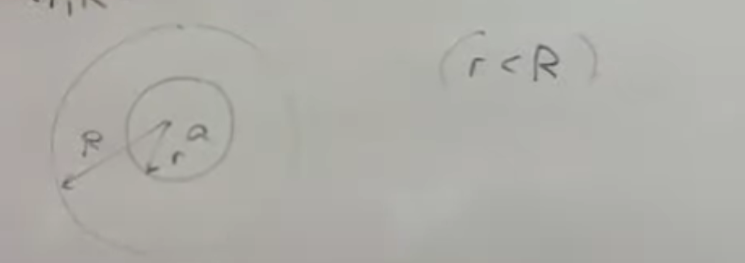
\includegraphics[scale=0.6]{img/convergence_ring_Laurent_series.png}

$a \in \C; f \in mathrm{Hal} \left(mathcal R _{r, R} (a)\right)$, где $-\infty \leqslant r < R \leqslant +\infty \implies \exists $ едиственный $(C_k)_{k\in \Z}\subset \C $:
\[\forall z \in \mathcal{R}_{r, R}(a),~~~~
f(z) = \sum_{k\in\Z} c_k (z 0 a )^k.
    \]

$c_k = \dfrac{1}{2\pi} \cdot \oint_{|z -a | \rho } \dfrac{f(z)}{(z - a) ^{k + 1}},~~~\rho \in (r, R) $.

\begin{definition}
    $a \in \overline{\C}$ называют изолированной особой точке $f(z)$, если $\exists$ окрестность $U(a)$:
    \[ f(z) \in \mathrm{Hol}(\overset{\cdot } {U} (a)). \]
\end{definition}
\begin{example}
\begin{enumerate}
    \item $f(z) = z$,~~~ $A = \{\infty  \}$.
    \item $f(z) = \overline{z}$,~~~ $ A = \O$ (все точки дифференцируемы).
    \item $f(z ) = \dfrac{1}{2} \left( z + \dfrac{1}{z} \right)$,~~~ $A = \{ 0, \infty\}$.
\end{enumerate}
\end{example}


\begin{definition}
    Пусть $a \in \overline{\C}$~--- и.о.т. $f(z)$. Тогда $a$ называется
    \begin{itemize}
        \item Полюсом $\iff \exists \lim_{z\to a} f(z) = \infty$.
        \item Существенно особой $\iff \not \exists \lim_{z\to a} f(z)$.
    \end{itemize}
\end{definition}

\begin{example}
\begin{enumerate}
    \item $f(z) = z$,~~~ $A = \{\infty  \}$, $\infty$~--- полюс.
    \item $f(z) = \dfrac{1}{2} \left( z + \dfrac{1}{z} \right)$,~~~ $A = \{ 0, \infty\}$, $0$ и $\infty$~--- полюсы.
    \item $f(z) = e^z$, ~~~ $A = \{\infty\}$,~~~ $\infty$~--- существенно особая точка.
\end{enumerate}
\end{example}

\begin{statement}
    Пусть $a\in \C, ~~~a$~--- и.о.т. $f(z)$. $\exists R~: f \in \mathrm{Hol}\left( \overset{\cdot}{B}_R (a) \right)$.\\
    Пусть $f (z) = \underbrace{\sum_{k = 0}^{+\infty } c_k (z - a)^k}_{\text{регулярная часть}} + \underbrace{\sum_{k \in -\N} c_k (z - a)^k}_{\text{главная часть лорановского разложения } f(z) \text{при} z \to a}$ ~~$\forall z \in \overset{\cdot}B_R (a)$.
\end{statement}

\begin{example}
    $f (z) = \dfrac{1}{1- z}$.

    В точке $z = 0$. Так как $f(z ) \in \mathrm{Hol} \left(B_1 (0) \right) \implies f(z) = \sum_{k = 0}^ \infty z^{k},~~~\forall z \in z \in B_1 (0)$.  Регулярная часть есть, а главная отсутствует.

    В точке $z = 1$. $f(z) = (-1) (z - 1)^{-1}$~--- главная часть.

    $z$ в окрестности $\infty$ $\dfrac{1}{1 - z } = \left( \dfrac{-1}{z} \right) \cdot \dfrac{1 }{ 1 - \dfrac{1}{z}} = \left(-1 \dfrac{1}{z} \right) \cdot \sum_{k=0}^\infty \left( \dfrac{1}{z} \right)^k$. Все регулярная часть, главная отсутствует.
\end{example}

\begin{statement}[Характеристика изолированных особых точек в терминах Лорановского разложения]

Пусть $a \in \overline{\C}$, ~~~$a$~--- и.о.т. $f(z)$. Тогда
\begin{enumerate}
    \item $a$~--- устранимая $\iff \exists $ окрестность $U(a)~:~ f \big|_{\overset{\cdot}{U} (a)}$~--- ограниченная $\iff$ главная часть лорановского разложения отстутствует.
    \item $a$~--- полюс $\iff $ главная часть лорановского разложения $f(z)$ в окрестности $a$ содержит конечное число членов.
    \item $a$~--- существенно устранимая $\iff$ главная часть лорановского разложения $f(z)$ содержит бесконечное число слогаемых.
\end{enumerate}
\end{statement}

Неравенство Коши ~:~$f(z) = \sum_{k \in \Z} c_k (z - a)^k, ~~~a \in \C$. $M_r = \sup_{z ~:~ |z - a | = r} |f| $,~~~ $ |c_k| \leqslant \dfrac{M_r}{r^k}$, $\forall k \in \Z$.

\begin{proof}
    ...
\end{proof}


\begin{note}
    Если $a \in \C$~--- и.о.т., то $\exists A~:~ \tl f (z) = \begin{cases}
        f(z),~~ z \neq a\\ A.
    \end{cases} \in \mathrm{Hol } (U(A))$.

    $f (z) = \sum_{k=0}^\infty c_k (z - a)^k$ в проколотой окрестности $a$.

    Проще говоря, можно исправить функцию в плохих точках и она станет хорошей.
\end{note}

\begin{example}
    $f(z) = \frac{sin z}{z} \in \mathrm{Hol}\left( \R \setminus \O  \right) $

    $f(z) = \frac{1}{z}\cdot \left( z - \frac{z^3}{3!}  + \frac{z^5}{5!} - \ldots \right) = 1 - \frac{z^2}{3!} + \frac{z^4}{5!} - \ldots$ -- сходится всюду в $\C$.
    Значит это продолжение функции $\frac{sin z}{z}$
\end{example}

\begin{note}
    [Отступление]

    \begin{lemma}
        [О кратности нуля]

        $f(z)\in \mathrm{Hol}\left( B_k(a) \right) , a\in \C, R>0$

        $f(a) = 0$ Тогда $\exists N\in \N : f(z) = (z-a)^N\cdot g(z)$, где $g(z)\in \mathrm{Hol}(B_k(a)), g(a)\neq 0 \implies f(z) \sim A \cdot (z-a)^N$, где $A = g(a)$
    \end{lemma}

    $f(z) = \sum_{k=0}^{\infty} c_k(z-a)^k$ в окрестности точки $a$, $c_0 = 0$
\end{note}

% эта часть куда идёт?.............

\begin{note}
    Если точка $a\in \C$ -- полюс, то $\sphericalangle g(z) = \frac{1}{f(z)}\to 0, z\to a$,
    $a$ -- устранимая для $g(z) \implies g(z) = (z-a)^N \cdot \tl g(z)\quad \tl g(a) \neq 0, \tl g\in \mathrm{Hol}(\text{окрестности т.} a)$

    \begin{align*}
        f &= \frac{1}{g} = \frac{1}{(z-a)^N} \frac{1}{\tl g(z)}\\
        &= \frac{1}{(z-a)^N} \cdot \left( \sum_{k=0}^{\infty} b_k(z-a)^k \right)  \\
        &= \frac{b_0}{(z-a)^N} + \frac{b_1}{(z-a)^{N-1}} + \ldots \\
    .\end{align*}
\end{note}

\begin{definition}
    $\sqsupset  a\in \C$ -- полюс для $f(z), N\in \N $

    $a$ -- полюс порядка $N$ для $f(z) \iff f(a) \sim \frac{C}{(z-a)^N} \left( \iff f(z) = \frac{g(z)}{(z-a)^n} \text{ где } g(z) \text{голоморфна в некоторой окрестности точка a функция}, g(a)\neq 0\right) $

    Для бесконечных точекрассматриваем $g(w) = \frac{1}{f(w)}$
\end{definition}

\begin{note}
    Любой полюс обладает порядком.
\end{note}

\begin{example}
    \begin{enumerate}
        \item $f(z) = \dfrac{1}{2 } \cdot \left( z + \dfrac{1}{z} \right)$. Полюс $0$ имеет порядок 1, полюс $\infty$ имеет порядок 1. Полюсы с порядком 1 называют \textbf{простыми}.
        \item $f(z) = \frac{\cos z - 1}{z^2} = \frac{-\frac{z^2}{2} + \frac{z^4}{4!} - \ldots}{z^3} = - \frac{1}{2z} + \ldots$. $0$ -- простой полюс (порядок 1), $\infty $ -- существенно особая.

        \item $f(z) = \tg z$. $\left\{ \frac{\pi}{2} + \pi k \right\}_{k\in \Z }$

        $\tg z = \frac{\sin z}{\cos z} \sim \frac{}{ \frac{\pi}{2} - z}\quad z = \frac{\pi}{2}$.  $\implies $ эти точки простые особые. $\infty $ -- не изолированная особая.
    \end{enumerate}
\end{example}

\begin{note}
    Почему может быть полезно знать какие особенности у функции в конкретной точке?
\end{note}

\begin{definition}
    $\sqsupset a\in \tl \C, a$ -- изолированная особая точка $f(z)$

    \[
    \res_a f = \begin{cases}
        c_{-1}&, \text{коэффициент в Лорановском разложении} f(z) \text{в окрестности точки} a\in \C\\
        -C_{-1}&, \text{коэффициент в Лорановском разложении} f(z) \text{в окрестности} \infty , a=\infty \\
    \end{cases}
    .\]
\end{definition}

\begin{example}
    \begin{enumerate}
        \item $f(z) = \frac{1}{2}(z + \frac{1}{z})\quad \res_0f = \frac{1}{2}, \res_{\infty }f = -\frac{1}{2}$
        \item $f(z) = \frac{1}{z^2 - 1} = \frac{1}{(z-1)(z+1)} = \frac{\frac{1}{2}}{z - 1} - \frac{\frac{1}{2}}{z+1}$

        $\res_1f = \res_1 \frac{\frac{1}{2}}{z - 1} = \frac{1}{2}\quad \res_{-1}f = -1\quad \res_{\infty }f = 0$, т.к. $f$ -- чётная
    \end{enumerate}
\end{example}

\begin{note}
    Чем хороши вычеты?
\end{note}

$c_k$ -- коэффициенты лорановского разложения в окрестности точки $a$, $f\in \mathrm{Hol}(B_R^\circ(a))$

\[
    c_k = \frac{1}{2\pi i} \oint _{|z+a| = \rho} \frac{f(z)}{(z-a)^{k+1}}dz\quad \rho\in(0,R)
.\]

$\res_af = c_{-1} = \frac{1}{2\pi i} \oint _{|z-a| = \rho}f(z)dz$

\begin{theorem}
    [Коши о вычетах]

    Пусть $O$ -- кусочно-гладкая область в $\tl \C$

    $A$ -- конечное множество, $A\subseteq O, f\in \mathrm{Hol}\left( \tl O \setminus A \right) $ Тогда:
    \[
    \int_{\partial O}f(z)dz = 2\pi i \sum_{a\in A}\res_a f = 2\pi i \sum_{z\in O}\res_zf
    .\]
\end{theorem}

\begin{theorem}
    [о полной сумме вычетов]

    $\sqsupset A\ni \infty , A\subseteq \tl \C, A$ -- конечно

    $\sqsupset f\in \mathrm{Hol}\left( \C \setminus A \right) $ Тогда:

    \[
    \sum_{a\in A}\res_af = \sum_{z\in \tl \C}\res_zf = 0
    .\]
\end{theorem}
\begin{proof}
    $\sqsupset A_0 = A \setminus \{\infty \}$

    Т.к. $A_0$ -- конечно, то $\exists B_R(0) \supset A_0$

    \begin{align*}
        \oint_{|z| = R} f(z)dz &= \left( \sum_{a\in A_0} \res_af \right) \cdot 2\pi i  \\
        &= \left( -\res_{\infty }\cdot 2\pi i \right)  \\
    .\end{align*}
\end{proof}

Приёмы вычсления вычетов ($a$ -- изолированная особая точка $f(z)$):
\begin{enumerate}
    \item $a$ -- устарнимая особая точка.
    \begin{enumerate}
        \item $a\in \C \implies \res_a f = 0$
        \item $a = \infty \quad f(z) = C_0 + \frac{C_1}{z} + \frac{C_2}{z^2} + \ldots$

        $\lim_{z \to \infty} f(z) = C_0$

        $\lim_{z \to \infty} z\left( f(\infty ) - f(z) \right) = \res_{\infty }f  $
    \end{enumerate}
    \item $a\in \C$ -- полюс. Тогда:
    $f(z) = \frac{C_{-N}}{(z-a)^N} + \ldots + \frac{C_{-1}}{(z-a)} + C_0 + C_1(z-a) + \ldots$

    $\res_af = \frac{1}{(N+1)!} \left( z_0 a^N f(z) \right) ^{(N-1)}_{z=a}$

    Если полюс простой, то $\res_af = \lim_{z \to a} f(z)(z-a)$

    Частный случай: $f(z) = \frac{\varphi(z)}{\psi(z)}, \varphi, \psi\in \mathrm{Hol}, \varphi(a) \neq 0, \psi(a) = 0, \p \psi(a) \neq 0$

    $\res_af = \lim_{z \to a} \frac{\varphi(z)}{\psi(z)}(z-a) = \lim_{z \to a} \frac{\varphi(z)}{\frac{\psi(z) - \psi(a)}{z - a}} = \frac{\varphi(a)}{\p\psi(a)}$

    \[
    \res_af = \frac{\varphi(a)}{\p\psi(a)}
    .\]
    \item Теорема о полной сумме вычетов.
    \item Если $f(z)$ чётная функция, то $\res_af = - \res_{-a}f$, в частности $\res_0 = 0 = \res_{\infty }$
    \item Если $f(z)$ нечётная, то $\res_af = \res_{-a}f$
\end{enumerate}

\begin{example}
    \begin{enumerate}
        \item $\int_{|z-1| = 1} \frac{dz}{z^4 +1}$

        $z^4 = -1$

        $z_1, z_4$ -- простые полюсы. $\res_{z_1}f = \frac{1}{4z_1^3} = \frac{z_1}{4z_1^4}  = - \frac{z_1}{4}$

        $\res_{z_2}f = -\frac{z_2}{4}$
        \begin{align*}
            \int_{|z-1| = 1} \frac{dz}{z^4 +1} &= 2\pi i\left( \res_{z_1} f + \res_{z_4} f \right)  \\
            &= -\frac{\pi i}{2}(z_1 + z_4) \\
            &= - \frac{\pi i}{2}\sqrt{2}  \\
        .\end{align*}
    \end{enumerate}
\end{example}



Приложение теоремы о вычетах к вычислению определённых и несобственных интегралов.
\begin{enumerate}
    \item $\int_{-\pi}^{\pi} R(\cos\varphi, \sin\varphi)d\varphi = \oint_{|z| = 1} R\left( \frac{z + \frac{1}{2}}{2}, \frac{z - \frac{1}{2}}{2} \right) \frac{dz}{iz} $

    $z = e$
\end{enumerate}
%% строчка

\begin{lemma}
    [Жордана]
    Пусть $f$ непрерывна в $|z| > R_0, \Im z > 0 \}$.
    $M(R) = \sup\left\{ |f(z) ~:~ z : |z| = R, \Im z \geqslant \right\}|$, $\Gamma _R = \{ |z | = R, \Im z \geqslant 0\}$

    Если $M(R) \to 0$, то $\forall m > 0 ~~~\int_{\Gamma_R} f(z) e ^{\Im z dz} \underset{R \to +\infty}{\to} 0 $.

\end{lemma}
% какое-то доказательство

\begin{lemma}
    [О полувычите]

   Пусть $\Gamma = \{ a + r  e ^{i\phi } _{\phi \in [\phi_0, \phi_0 + \pi]}$.
   $a \in \C$~--- простой полюс $f(x)$.

   Тогда $\int_{\Gamma(r)} f (z) dz \underset{r \to 0_+}{\to} \pi i res_a f $.
\end{lemma}

\begin{proof}

    При достаточно малых $r$, т.к. $a$ -- простой множитель
    \begin{align*}
        \int_{\Gamma(r)} f(z)dz &= \int_{\Gamma(r)} \frac{C_{-1}}{z-a} + \overbrace{\sum_{k=0}^{\infty } C_k (z-a)^k}^{\varphi(z)} dz\\
        &= \overbrace{C_{-1}}^{\res_a f} \underbrace{\int_{\Gamma(r)}}_{I_1} \frac{dz}{z-a}  + \overbrace{\int_{\Gamma(r)}\varphi(z) dz}^{J}\\
        I_1 &= \int_{\varphi_0}^{\varphi_0 + \pi} \frac{ire^{i\varphi}d\varphi}{re^{i\varphi}} = \pi i \\
        |J| \leqslant C\cdot \pi r \to 0\quad r\to 0
    .\end{align*}
\end{proof}


\section{Интегралы в смысле главного значния}
Пусть $f \in C\left([a, b] \setminus c) \right)$, $c \in (a, b)$.

\[
v.p. \int_a^b f(x) dx  = \lim_{\varepsilon \to 0^+ } \left(
    \int_a^{c - \varepsilon} f(x) dx + \int_{c + \varepsilon}^b f(x)dx \right).
\]

Особенных точек может быть много, поэтому там может возникнуть нескольк таких пределов.

\begin{example}
    $\int_0^{+\infty} \dfrac{\sin x}{x} dx = I$.

    \begin{align*}
        I &= \dfrac{1}{2} \int_{-\infty}^{infty} \frac{\sin x}{x} \\
        &= \frac{1}{2} v.p. \int _{-\infty }^{\infty } \frac{\overbrace{\sin x}^{\Im e^{ix}}}{x}dx\\
        &= \frac{1}{2} v.p. \frac{1}{i} \int_{-\infty }^{\infty } \frac{\cos x + i\sin x}{x}dx\\
        &= \frac{1}{2i} \pi i = \frac{\pi}{2}\\
    .\end{align*}


    $\frac{\cos x}{x}$ -- нечётная функция, значит интеграл в смысле главного значения по области без особых точек сходится и равен 0.
\end{example}


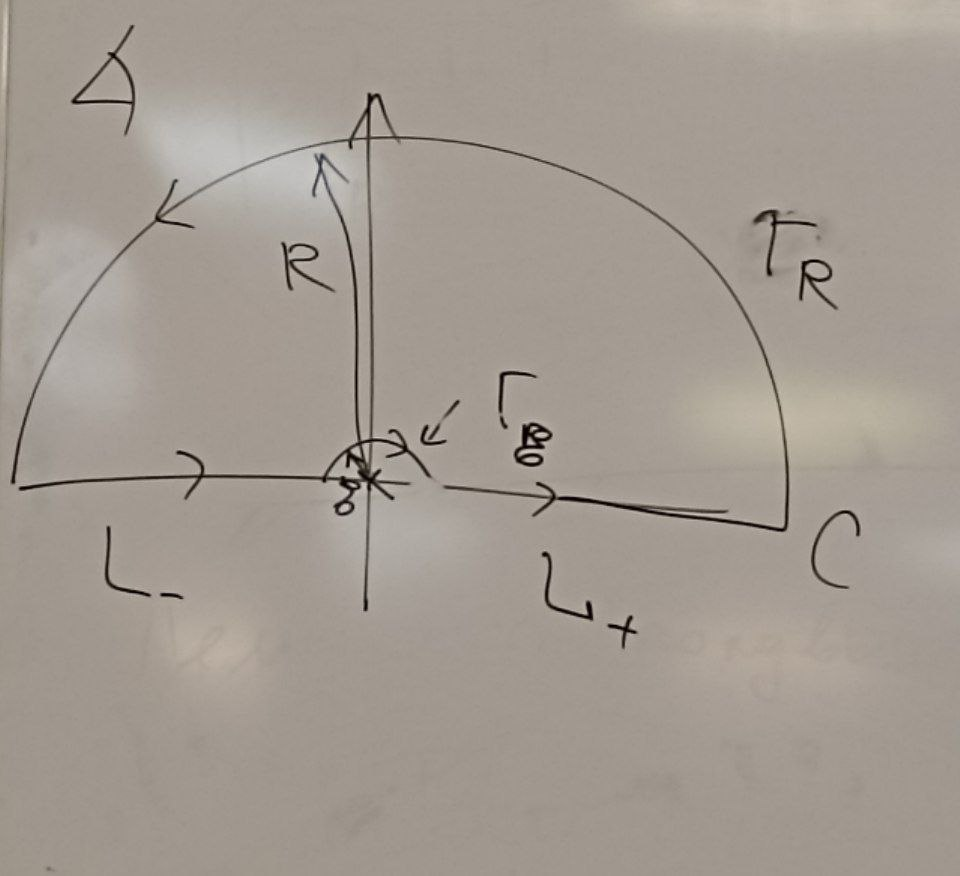
\includegraphics[scale=0.17]{img/obgod_vp.jpg}

$\sphericalangle $ контур из двух верхних полуокружностей с радиусами $R,\varepsilon$ и прямыми вдоль оси $Ox$, соединяющими их, обходимый против часовой стрелки.

\begin{align*}
    0 = \int _C \frac{e^{iz}}{z}dz = \underbrace{\int_{\Gamma_R}fdz}_{\to 0 \text{;Жордан}} + \overbrace{\int_{\Gamma_{\varepsilon}}fdz}^{-\pi i \res_0 f} + \int _{L_+}fdz + \int_{L_-}fdz\\
    v.p. \int_{-\infty }^{\infty }f(x)dx = \pi i \res_0f = \pi i
.\end{align*}


\section{Возвращение к дифферецниальным формам}

\begin{definition}
    $\omega$ -- замкнутая формула если $d\omega = 0$
\end{definition}

\begin{definition}
    $\omega$ -- точная в области $O$, если существует форма $\Omega$ -- дифферецниальная форма в области $O$, т.ч. $d\Omega = \omega$
\end{definition}

\begin{lemma}
    Точноасть влечёт засмкнутость. Потому что $d(d(\Omega)) \equiv 0$
\end{lemma}

\begin{lemma}
    Если $\omega$ замкнута в шаре $B(a) \subseteq \R^n$, то она там точна.
\end{lemma}

\begin{note}
    Если $\omega$ -- точная 1 форма, $\omega = dF \implies \int_\gamma \omega = F\mid_{\gamma(a)}^{\gamma(b)}$, если $\gamma: [a,b] \to \R^n$

    $\int_\gamma \omega = \int_a^b \underbrace{dF \circ \gamma(t)\cdot \p \gamma(t)}_{\p{F(\gamma(t))}} dt = F(\gamma(t))_a^b$

    Инетграл не зависит от пути, соединаяющего точки $a$ и $b$
\end{note}

\begin{proof}
    [проверка леммы для 1-форм, $n=2$]

    $F(p) = \int_{\vec{a,p}}\omega$

    $\omega = Pdx + Qdy\quad \p p = \p Q_x - \p P_y dxdy$

    Рассмотрим контур по прямоугольному треугольнику с гипотенузой $ap$. Интеграл по этой этому контуру равен 0. По формуле Грина:
    \[ 0 = \int_{\partial O_1} = -\int _{ap}\omega + \int_{aq}\omega + ]int_{qp}\omega\]

    \begin{align*}
        F(x,y) = F(p) &= \int_{a}^q\omega + \int_q^p\omega = \int_{x_0}^{x} P(t,y_0)dt + \int_{y_0}^yQ(x,s)d\\
        \p F_x(x,y) = P(x,y_0) + \int_{y_0}^y \underbrace{\p Q_{x}(x,s)}_{\p P_y(x,s)}ds = P(x,y)\\
        \p F_y(x,y) = Q(x,y)\\
    .\end{align*}

    Следовательно $F$ -- первообразная для $f$ в круге $B_R(a)$


\end{proof}

\begin{theorem}
    [Пуанкаре]

    Всякая замкнутая в (односвязной) выпуклой области точна в этой области.
\end{theorem}

\begin{proof}
    [показательство ]

    $\Phi(p) = \int_{ap}\omega$

    $\Phi(p) = \int_{ap_1}\omega + \int_{p_1p}\omega\quad \p\Phi(p) = \Phi_1(p) = \omega\;\forall p\in B_R(p_1)$
\end{proof}

\begin{problem}
    $\int_0^{+\infty } \frac{\sin^2 x}{x^2}dx\quad \sphericalangle \frac{e^{2it} - 1}{z^2}$
\end{problem}

\begin{note}
    Существуют замкнутые, но не точные дифференциальные формы.
    \[ w = \dfrac{x dy - y dx}{x^2 },~~~~
    w = d\left(\dfrac{y}{x} + C\right), x > 0.\]

    \[w = \dfrac{x dy - y dx}{x^2 + y^2} = \dfrac{x dy - y dx}{y^2} \cdot \dfrac{1}{1 + \left(\dfrac{x}{y}\right)^2},~~~~((x, y)\neq 0, )\]
    \[ \oint_{|(x, y)| = R} \dfrac{x dy -y dx}{x^2 + y^2} = \int_{-\pi}^{\pi} \dfrac{R^2 \left(\cos^2 \phi + \sin^2 \phi \right)}{R^2} = 2\pi \neq 0 \implies\]
    $w$ не точна в $\R^2 \setminus(0, 0)$.

\end{note}

\section{Пространства $L^p(X, \mu), e^p$}

\begin{note}
    Неравенство Минковского:
    \begin{itemize}
        \item для сумм $x_1, \ldots, x_k\quad y_1, \ldots, y_k \in \R\quad p \geqslant 1$

        \[()\sum_{k=1}^{K} |x_k + y_k|^p)^{\frac{1}{p}} \leqslant \left( \sum_{k=1}^{K} |x_k|^p \right)^{\frac{1}{p}} + \left( \sum_{k=1}^{K} |y_k|^p \right)^{\frac{1}{p}} \]
        \item $\left( \int_a^b |f + g|^p \right) ^{\frac{1}{p}} \leqslant \ldots\qquad f, g\in C([a,b])$
    \end{itemize}
\end{note}

\begin{theorem}
    $\sqsupset (X, \mu)$ -- пространство с мерой, $f, g\in \mathcal L(X, \mu)$

    \[\left( \int_X |f+g|^pd\mu \right) ^{\frac{1}{p}} \leqslant \left( \sum_{k=1}^{K} |f|^p \right)^{\frac{1}{p}} + \left( \sum_{k=1}^{K} |g|^p \right)^{\frac{1}{p}}\]
\end{theorem}
\begin{proof}
    \begin{enumerate}
        \item $f,g$ -- ступенчатые и неотрицательные. Тогда существует общее допустимое разбиение $\{E_k\}_{k=1}^K\quad X = \coprod_{k=1}^KE_k\qquad f\mid_{E_k} \equiv f_k\quad g\mid_{E_k}\equiv g_k$ -- числа, постоянные

        $f(x) = \sum_{k=1}^{K} f_k \chi_{E_k}(x)\qquad g(x) = \sum_{k=1}^{K} g_k\chi_{E_k}(x)$

        $\int_X |f+g|^pd\mu = \sum_{k=1}^{K} \int_{E_k}|f + g|^pd\mu = (f_k + g_k)^p \cdot \underbrace{\mu(E_k)}_{m_k}$

        $x_k = f_k m_k^{\frac{1}{p}}\quad y_k = g_k m_k^{\frac{1}{p}}$

        $\left(\int_X |f+g|^pd\mu  \right)^{\frac{1}{p}}$($ (A)!(B)!(C) $)
    \end{enumerate}
\end{proof}


\begin{proof}
    \begin{enumerate}
        \item $f,g$ -- ступенчатые и неотрицательные. Тогда существует общее допустимое разбиение $\{E_k\}_{k=1}^K\quad X = \coprod_{k=1}^KE_k\qquad f\mid_{E_k} \equiv f_k\quad g\mid_{E_k}\equiv g_k$ -- числа, постоянные

        $f(x) = \sum_{k=1}^{K} f_k \chi_{E_k}(x)\qquad g(x) = \sum_{k=1}^{K} g_k\chi_{E_k}(x)$

        $\int_X |f+g|^pd\mu = \sum_{k=1}^{K} \int_{E_k}|f + g|^pd\mu = (f_k + g_k)^p \cdot \underbrace{\mu(E_k)}_{m_k}$

        $x_k = f_k m_k^{\frac{1}{p}}\quad y_k = g_k m_k^{\frac{1}{p}}$
        \begin{align*}
            \left(\int_X |f+g|^pd\mu  \right)^{\frac{1}{p}} &= (\sum_{k=1}^{K} \int_{E_k}(f+g)d\mu) \\
            &\leqslant \left(\sum_{k=1}^{K} f_k^p m_k \right)^{\frac{1}{p}} + \left(\sum_{k=1}^{K} g_k^p m_k \right)^{\frac{1}{p}} \\
            &= \int_Xf^pd\mu + \int_X g^pd\mu \\
        .\end{align*}
        \item $f,g$ -- неотрицательные, измеримые. Они приближаются последовательностями ступенчатых.

        \item $f,g$ -- комплеснозначные

        \[\left(\int_X |f+g|^pd\mu  \right)^{\frac{1}{p}} \leqslant \left( \int_X \left( |f| + |g| \right)^pd\mu  \right)^{\frac{1}{p}} \leqslant \text{неравенство для модуля}  \]
    \end{enumerate}
\end{proof}

\begin{note}
    Аналогично неравенство Гёльдера $p, q > 1\quad \frac{1}{p} + \frac{1}{q} = 1$

    \[\int_X |fg|d\mu \leqslant \left( \int_X|f|^pd\mu \right) ^{\frac{1}{p}} \left( \int_X |g|^qd\mu \right) ^{\frac{1}{q}}\]
\end{note}

\begin{definition}
    \[\mathrm{esssup}_x f = \inf \{M\in \R: \text{ для п.в. } x\in X]quad f(x)  \leqslant M\}\]

    существенный супремум.
\end{definition}

$f\sim g \iff f = g$ почти везде на $X$

$g\sim f \implies \|f\|_p = \|g\|_p$

\begin{definition}
    \[L^p(X, \mu) = \left\{ [f]: \|f\|_p <+\infty  \right\} \]

\end{definition}

\begin{statement}
    Если $\mu(X) <+\infty $, то $L^p(X, \mu)$ ``убывает'' по $p$

    $\tl p > p \geqslant 1 \implies L^{\tl p}(x, \mu) \subseteq L^p(X, \mu)$

    $L^{\infty }(X, \mu) \subseteq \ldots L^2(X, \mu) \subseteq L^1(X, \mu)$

    $C^0([a,b]) \subseteq L^{\infty }([a,b]) \subseteq \ldots \subseteq L^2([a,b]) \subseteq \ldots \subseteq L^1([a,b])$
\end{statement}

Если $\mu(X) = +\infty $, то $L^2(\left<a,b \right>) \nsubseteq\nsupseteq$

\begin{enumerate}
    \item $f(x) = \chi_{(1, +\infty )}(x) \frac{1}{x} \in L^2(\R)\setminus L^1(\R)$
    \item $f(x) = \chi_{(0,1)}(x) \frac{1}{\sqrt{x} }\in L^1(\R) \setminus L^2(\R)$
\end{enumerate}

\begin{statement}
    $f\in L^{\tl p} \implies f\in L^p\qquad \tl p > p \geqslant 1$
\end{statement} %я тут пропустил докво, потому что руки устали

\begin{note}
    Факт:
    \begin{enumerate}
        \item $\forall p\in [1, +\infty]\;\;L^p(X, \mu)$ полно, $C([a,b])$ плотно в $L^p([a,b])$
        \item $C([a,b])$ плотно в $L^p({a,b}) \;\forall p\in [1,+\infty ]$
    \end{enumerate}
\end{note}

\begin{definition}
    \[l^p = L^p(\N , \nu)\]

    $l^p = \begin{cases}
        \{(x_k)_{k=1}^{\infty }: \sum_{k=1}^{\infty } |x_k|^p <+\infty \}\\
        \{x = (x_k)_{k=1}^\infty \text{ -- огр}
    \end{cases}$

    $l^p$ ``возрастает'' по $p$
\end{definition}

\begin{definition}
    [Скалярное произведение в $L^2(X, \mu)$]

    $\left<f,g \right> = \int_Xf \cdot \overline gd\mu$

    По неравенству Гёльдера этот интеграл конечен.

    $\|f\|_2 = \sqrt{\left<f,f \right>} $
\end{definition}

\begin{definition}
    $f_j\in L^2(X, \mu)$ -- счётное множество, $f_i \neq 0$ в  $L^2\quad f_j\perp f_k$ при $j\neq k$

    Тогда $\{f_j\}$ называется ортогональной системой

    ОНС $\|f_j\| = 1$
\end{definition}

\begin{example}
    $L^2[-\pi, \pi]\quad f_j(t) = e^{ijt}$

    \begin{align*}
        \left<f_j, f_k \right> &= \int_{-\pi}^{\pi} e^{ijt}e^{-ikt}dt \\
        &= \int_{-pi}^{\pi}e^{i(j-k)t}d\mu \\
        &= \begin{cases}
            2\pi&k=j\\
            \frac{e^{i(j-k)t}}{i(j-k)t}\mid_{-\pi}^{\pi} = 0
        \end{cases} \\
    .\end{align*}
\end{example}

%%%

$\int_{-\pi}^\pi \cos k t \cos jt dt = \begin{cases}
    0, & k\neq j\\
    \pi, & k = j \neq 0\\
    2\pi, & k =j = 0
\end{cases}$; $\int_{-\pi}^\pi \sin k t a\sin j t dt = \begin{cases}
    0, & k\neq j\\
    \pi, & k = j
\end{cases}$, где $k, j \in \N$.

Ортагональная Нормальная система: $\left\{ \dfrac{1}{\sqrt{2}\pi}, \dfrac{1}{\sqrt{\pi}}\cos t, \dfrac{1}{\sqrt{\pi}}\sin t,
\dfrac{1}{\sqrt{\pi}} \cos 2t, \dots
\right\}$.
\begin{definition}
    Многочлены Чебышёва 1-го рода
    \[T_n(t) = \cos(n \arccos t)\quad t\in [-\pi, \pi]\;\; n\in \Z_+\]

    $L^2([-1,1], \frac{1}{\sqrt{1}{1 - t^2}})$
\end{definition}

\begin{note}
    $L^p, (X, \mu)$ -- полно, $\forall p \in [1, +\infty ]$

    $C[-\pi, \pi]$ -- плотно в $L^p[-\pi, \pi]$

    $\forall \varepsilon >0 \forall f\in L^p[-\pi, \pi]\; \exists g\in [-\pi, \pi]: \|f - g\|_p <\varepsilon$
\end{note}

\begin{note}
    $\sqsupset \{f_k\}_{k=1}^{\infty } \subseteq L^p[a,b]\quad f_k \to f$ в $L^p$

    Иначе: $\|f_k - f\|_p \to 0, k\to \infty$. $\implies f_k \to f, k\to \infty $ почти везде на $[a,b]$
\end{note}

\begin{note}
    $L^2\left( [a,b], \mu \right) $

    $\left<f, g \right> = \int_{[a,b]}f \cdot \ov g d\mu$ -- скалярное пространство в $L^2([a,b], \mu)$
\end{note}

\begin{definition}
    Полное линейное пространство со скалярным произведением называется Гильбертовым.
\end{definition}

\begin{example}
    $L^2(X, \mu)\quad l^2$

    $x = (x_k)_{k=1}^{\infty }\quad y = (y_k)_{k=1}^{\infty }\quad \left<x,y \right> = \sum_{k=1}^{\infty }x_k \ov y_k$
\end{example}

\begin{note}
    $\forall y \in H$\\
    $\varphi(x) = \left< x, \ov y \right>$~--- непрерывно из $H$ в $\R$ (в $\C$)

    $| \varphi(x_1) - \varphi(x_2)| = |\left< x_1 - x_2 , y \right> \leqslant \| x_1 - x_2\| \|y\|$~--- липшицево с константой $\|y\|$.
\end{note}

\begin{note}
    $\sqsupset \sum_{k=1}^{\infty } x_k $ -- сходящийся ряд в Гитбертоом пространстве $\mathcal H$. Тогда $\forall y\in H$
    \[ \left< \sum_{k=1}^{\infty } x_k, y \right> = \sum_{k=1}^{\infty }\left<x_k, y \right> \]
\end{note}

\begin{note}
    $\varphi(x) = \left<x,y \right>$

    $\varphi\left(\underbrace{\sum_{k=1}^{\infty } x_k }_{\lim S_n } \right) = \lim_{n \to \infty} \varphi(S_n) = \lim_{n \to \infty} \sum_{k=1}^{n } \left<x_k, y \right> = \sum_{k=1}^{\infty } \left<x_k, y \right> $

    $S_n = \sum_{k=1}^{n} x_k$
\end{note}

\begin{theorem}
    [<<Пифагора>>]

    Пусть $\{ x_k\}_{k=1}^\infty$~--- о.с. в Гильбертовым пространстве $\mathcal{H}$. Тогда

    \begin{enumerate}
        \item $\forall n \in \N$
        \[ \left\|\sum_{k=1}^n x_k \right\|^2 = \sum_{k =1}^n \|x_k\|^2. \]
        \item $\sum_{k=1}^\infty x_k$ сходится в $\mathcal{H} \iff \sum_{k =1 }^\infty \|x_k\|^2$ сходится
        случае сходимости $\left\| \sum_{k=1}^\infty x_k \right\|^2 = \sum_{k=1}^\infty \|x_k\|^2$.
    \end{enumerate}
\end{theorem}

\begin{proof}
    \begin{enumerate}
        \item $\left\| \sum_{k=1}^n x_k \right\| = \left< \sum_{k=1}^n x_k, \sum_{k=1}^n x_k \right> = \sum_{k=1}^n \left< x_k, \sum_{j=1}^n x_j\right> = \sum_{k=1}^n \| x_k\|^2$.
        \item $S_n = \sum_{k=1}^n x_k$, $\tl{S}_n = \sum_{k=1}^n \|x_k \| ^2$.

        \[ \|S_n - S_m\|_{n > m}^2 = \left\| \sum_{k = m + 1}^n x_k  \right\|^2 = \sum_{k = m + 1}^n \| x_k\|^2 = \tl S_n - \tl S_m = | \tl S _m - \tl S_n| \implies  \]
        $(S_n)$~--- сходится  $\iff$ $ S _n$~--- фундамнтальная $\iff$ $\tl S _n$~--- фундамнтальная $\iff$ $\tl S_n$~--- сходится

        Если $\sum x_k$ сходится
        \[ \left\| \sum_{k=1}^\infty x_k  \right\|^2 = \lim_{n\to\infty} \left\| \sum_{k=1}^n x_k \right\| = \lim_{n \to \infty } \sum_{k=1}^n \| x_k \| ^2 =\sum_{k=1}^\infty \|x_k\|^2 \]
    \end{enumerate}
\end{proof}

Пусть  $x \in \mathcal{H}$, $\{ e_k\} _{k=1}^\infty$~--- ортагональная система в $\mathcal{H}$.

Пусть $x = \sum_{k = 1}^\infty c_k e_k$, $c_k$~--- скаляр. Тогда
\[c_k = \dfrac{\left< x, e_k \right>}{\|e_k\| ^2}~~~~ \forall k \in \N
    \]

Пусть $k \in \N$~~~$\left< x, e_k \right> = \left< \sum_{y = 1}^\infty e_k e_j, e_n \right>  =$

\begin{example}
    \begin{enumerate}
        \item $l^2 = \left\{ \left( x_1, x_2, \ldots, x_k, \ldots \right) ) : \sum_{k=1}^{\infty } |x_k|^2  \right\}$

        $e_1 = (1,  0, \ldots)\quad e_2 = (0, 1, , \ldots), \ldots$

        $\left<e_j, e_k \right> = \delta_{jk}$

        $c_k = \left<x, e_k \right> = x_k$

        $x = \sum_{k=1}^{\infty } x_ke_K\quad \sum_{k=1}^{\infty } x_k^2 <\infty  $

        $\{e_k\}_{k\geqslant k_0}$ -- ортонормированная система
    \end{enumerate}
\end{example}

\begin{theorem}
    [О свойствах конечных сумм рядов Фурье]

    $\sqsupset \mathcal{H}$ -- Гильбертово пространство. $x\in H\quad \{e_k\}$ -- ортонормированны в $\mathcal{H}$. $S_n = \sum_{k=1}^{\infty } c_k e_k$

    $\forall  n\in \N $
    \begin{enumerate}
        \item $x = s_n + z_n]\quad z_n \perp \mathcal L_{in} \{e_1, e_2,\ldots e_n\} = \mathcal L_n$

        Т.е. $S_n$ -- ортогональная проекция $x$ на $L_n$
        \item $AA y\in \mathcal L_n$ \[ \|x-y\| \geqslant \|x - \delta_n\|\]
        Пишем равенство только в условии, что $y = S_n$

        Т.е. $S_n$ -- единственный элемент наилучшего приближения к $x$
        \item $\|S_n\| \leqslant  \|x\| \iff \sum_{k=1}^{n} |C_k|^2 \|e_k\|^2 \leqslant \|x_k\|^2$ -- неравенство Бесселя
    \end{enumerate}
\end{theorem}
\begin{proof}
    $z_n = x - S_n$

    $\sqsupset j\in \{1, \ldots, n$

    \begin{align*}
        \left<z_n, e_j \right> &= \left<x, e_j \right> - \left<S_n, e_j \right>\\
        &= \left<x, e_j \right> - e_j \left<e_j, e_j \right> = 0  \\
        \implies & z_n \perp e_j \implies z_n \perp \mathcal L_n\end{align*}

    \begin{align*}
        \|x - y\|^2 &=  \|S_n + z_n - y\|^2 \\
        &= \|\underbrace{\left( S_n - y \right)}_{\in \mathcal L_n}  + \underbrace{z_n}_{\perp z\mathcal L_n}\|^2 \\
        &= \|S_n - y\|^2 + \|z_n\|^2 \\
        &\geqslant \|z_n\|^2 = \|x - S_n\|^2\\
    .\end{align*}

    \begin{align*}
        \|x\|^2 &= \|S_n + z_n\|^2 = \|S_n\|^2 + \|z_n\|^2\\
        &\geqslant \|S_n\|^2 \\
    .\end{align*}

    Неравенство Бесселя -- результат применения теоремы Пифагора.
\end{proof}

\begin{theorem}
    [Рисса-Фишера]

    $\sqsupset \mathcal{H}$ -- г.п., $\{e_k\}$ -- ОС в $\mathcal{H}, x\in \mathcal{H}$

    \begin{enumerate}
        \item Ряд Фурье \[\sum_{k=1}^{\infty } C_ke_k:\quad c_k \text{ коэффициент Фурье }\]
        сходится
        \item $x = \sum_{k=1}^{\infty } C_K e_k + z\quad z\perp e_j \forall j $
        \item $x = \sum_{k=1}^{\infty } C_k e_k \iff \sum_{k=1}^{\infty } |C_k|^2 \|e_k\|^2 = \|x\|^2 $\\--- Тождество Бесселя (Равенство Парсеваля, уравнение замкнутост)
    \end{enumerate}
\end{theorem}
\begin{proof}
    По теореме Пифагора сходимость ряда Фурье равеносильно
    \[ \sum_{k=1}^{\infty } \|C_k e_k\|^2 = \sum_{k=1}^{\infty } |C_k|^2 \|e_k\|^2 \leqslant \|x\|^2. \]

    Здесь в конце предельный переход по неравенству Бесселя. Раз частичные суммы ограничены, то ряд сходится.

    $z = x - \sum_{k=1}^{\infty }c_ke_k $

    \begin{align*}
        \left<z, e_j \right> = \left<x, e_j \right> - \left<\sum_{k=1}^{\infty } C_ke_k, e_j  \right>\\
        &\left<x, e_j \right> - \sum_{k=1}^{\infty } C_k\left<e_k, e_j  \right> = 0 \\
    .\end{align*}

    $x = \underbrace{\sum_{k=1}^{\infty }C_ke_k}_S \iff z = 0 $

    $x = S + z\quad S\perp z$

    $\|x\|^2 = \|S\|^2 + \|z\|^2 \implies \left( \|x\|^2 = \|S\|^2 \iff x = S \right) $
\end{proof}

\begin{definition}
    ЛНЗ система $\{x_k\}_k$ -- базис в нормированном пространстве $X$, если
    \[\forall x\in X \exists \{x_k\}_{k=1}^{\infty } \subseteq \R(\C); x = \sum_{k=1}^{\infty } c_k x_k \]
\end{definition}

\begin{definition}
    ОС $\{e_k\}_{k=1}^{\infty }$  в Гильбертовом пространстве $H$ называется замкнутой, если $\forall x\in H$ верно уравнение замкнутости:
    \[\|x\|^2 = \sum_{k=1}^{\infty } |c_k|^2 \|e_k\|^2, \]

    где $c_k$~--- коэффициент Фурье по системе из $\{ e_k \}$.
\end{definition}

\begin{definition}
    $\sqsupset \{e_k\}$ -- ОС в $H$. Она называется полной, если $\nexists z\in H \setminus \{0\}:\quad z\perp e_i \forall \in \N $.
\end{definition}

\begin{theorem}
    $\sqsupset \{e_k\}$ -- ОС в г.п. $H$. Следующие утверждения равносильны:
    \begin{enumerate}
        \item $\{e_k\}$ -- базис
        \item $\forall x, y\in H$
        \[ \left<x, y \right> = \sum_{k=1}^{\infty } c_k(x) \cdot \ov {c_k (y)}\cdot \|e_k\|^2 \]

        $c_k(t)$ -- коэффициент Фурье по системе $e_k$
        \item $\{e_k\}$ -- замкнута
        \item $\{e_k\}$ -- полная
        \item $\left\{\sum_{j=1}^{n} c_j e_j: c_j\in \R(\C)\right\}_{n\in \N }$ -- плотно в $H$
    \end{enumerate}
\end{theorem}

\begin{proof}
    \begin{enumerate}
        \item $1\implies 2$.

        $x = \sum_{k=1}^{\infty } C_k(x)e_k\quad y = \sum_{k=1}^{\infty }c_k(y)e_k$

        \begin{align*}
            \left<x,y \right> &= \left( \sum, \sum \right) \\
            &= \sum \left<c_k(x)e_k, \sum \right> \\
            &= \ldots \\
        .\end{align*}
        \item $2\implies 3$. Очевидно
        \item $3 \implies 4$. $\sqsupset \forall j\in \N \; z\perp e_j \implies c_k(z) = 0$

        $\|z\|^2 = \sum_{k=1}^{\infty }|c_k(z)|^2 \|e_k\|^2 = \sum 0 = 0 \implies \|z = 0\| \implies z = 0 $
        \item $4 \implies 1 $ $ \sphericalangle x = \sum_{k=1}^{\infty }c_k(x) \cdot e_k  + z$ -- по теореме Риса Фишера.
        $z \perp e_j$. В предположении $e_k$ полные, значит $z = 0 \implies e_k$ -- базис
        \item $1 \implies  5$

        $\forall \varepsilon>0 \forall x\in H\exists N\in \N \exists c_1, \ldots, c_N: \quad \|x - \sum_{k=1}^{N} c_ke_j\|<\varepsilon$

        По 1 $\sum_{k=1}^{\infty } c_ke_j \to x$ -- сходится, а значит разность с $x$ стремится к 0 и можно для $\forall \varepsilon$ подобрать нужное $N$
        \item $5 \implies 1$ $\sqsupset \varepsilon>0$
        $\|x - \sum_{k=1}^{n} \tl c_ke_k\ < \varepsilon$

        $\|x - \overbrace{S_N}^{\text{сумма Фурье}}\| \leqslant  \|x - \sum_{k=1}^{N} \tl c_k e_k\| < \varepsilon$

        $x - s_n = z_n\quad z_n\perp S_N$

        $x = s_N + z_n = s_N + \underbrace{(s_n - s_N)}_{\in \mathcal L\{e_{N+1}, \ldots, e_n\}} + z_n$

        $\|x - S-N\|^2 = \|S_n - S_N\|^2 + \|z_n\|^2$

        $\|x - S_n\|^2 = \|z_n\|^2$

        $\|x - S-N\|^2 \leqslant \|x - S_n\|^2$

        $\implies S_n \to x \implies \{e_k\} $ -- базис
    \end{enumerate}
\end{proof}

\section{Тригонометрические ряды Фурье}

$f \in L^1(-\pi, \pi]$

$|\left<f, g \right>| \leqslant \|f\|_1 \cdot \|g\|_{\infty } = \|f\|_1$

$f\in L^1\quad g = \cos kt, \sin kt, e^{ikt}$

$|\left<f, g \right>| = \int_{-\pi}^{\pi} f(t)\ov g(t)dt$

\begin{definition}
    \[\frac{a_0}{2} + \sum_{k=1}^{\infty } \left( a_k\cos kt + b_k\sin kt \right)  \]

    $a_k = \frac{1}{\pi}\int_{-\pi}^{\pi}f(t)\cos kt dt\quad k\in \Z_+$

    $b_k = \frac{1}{\pi} \int_{-\pi}^{\pi}f(t)\sin kt dt\quad k\in \N $

    $C_k(x) = \cos k x\quad S_k(t) = \sin kt$

    $k \geqslant 1\quad \|C_k\| = \|S_k\| = \pi$

    $a_k = \frac{\left<f, C_k(t) \right>}{\|C_k(t)\|}$

    $C_0 (t) = 1, ~~~c_0 \dfrac{\left< f, C_0(t) \right> }{\| C_0\|^2} = \dfrac{\left< \dots, \dots \right>}{2\pi} = \dfrac{a_0}{2}$.

    Ряд Фурье $ = c_0(f) + \sum_{k=1}^{\infty } c_k(f)\cos(kt) + b_k(f)\sin k t $
\end{definition}

\begin{note}
    [Факт]

    $\{\cos kt, \sin kt\}_{k\in \N } \cup \{1\}$ -- базис $L^2\left( [-\pi, \pi] \right) $

    $\forall f\in L62\quad f(x) = \frac{a_0(f)}{2} + \sum_{k=1}^{\infty } \left( a_k \cos kt + b_k\sin kt \right) $ -- почти везде равенство\ldots

    $\|f\|^2 = \frac{|a_0|}{2} + \left(\sum_{k=1}^{\infty } |a_k|^2 + |b_k|^2\right)^2 \pi \iff \frac{\|f\|}{\pi} = a_0^2 + \sum_{k=1}^{\infty }\left( |a_k|^2 + |b_k|^2 \right)  $
\end{note}

\begin{note}
    [Факт 2] Следствие признака Дини

    $\sqsupset  f\in L^1([-\pi, \pi])\quad f$ -- $2\pi$-периодическая

    $\sqsupset x\in \R$

    $\exists f(x+\pm 0)\in \R$ И $\lim_{t \to 0+} \frac{f(x+t) - f(x+0)}{t} \in \R $ и $\lim_{t \to 0-} \frac{f(x+t)- f(x-0)}{t}\in \R$

    Тогда в тех $x$, что тригонометрический ряд Фурье сходится.

    $S(x) = \frac{f(x+0) + f(x-0)}{2}$
\end{note}

\begin{example}
    $\sphericalangle 2\pi$-периодическое продолжение  $\mathrm{sign} x\quad f(\pi k) = 0 \implies f(x) \equiv S(x)$
\end{example}

\begin{note}
    Если $f\in L^1$ и $f$ нечётная, то $a_k = 0\quad b_k = \frac{2}{\pi}\int_0^\pi f(t)\sin kt\quad j\in \N $ и ряд Фурье будет содержать только синусы

    Если наоборот, то $b_k = 0\quad a_k = \frac{2}{\pi} \int_0^\pi f(t)\cos kt dt$
\end{note}

\begin{example}
    $a_k = 0$

    \begin{align*}
        b_k &= \frac{2}{\pi} \int_0^\pi \mathrm{sign}(t)\sin kt \\
        &= \frac{2}{\pi} \frac{\cos kt }{k}\mid _{\pi}^0 \\
        &= \frac{2}{\pi k} \\
    .\end{align*}
\end{example}




%%% NO
% oh well минус пол лекции потамушта интернет. Ладно там только примеры были
%пофиг) :checkmark: :thumbup:

\end{document}